\documentclass{article}

\usepackage{neurips_2026}

% Override Helvetica with Computer Modern Sans (helvetic not installed)
\renewcommand{\sfdefault}{cmss}

\usepackage[utf8]{inputenc}
\usepackage[T1]{fontenc}
\usepackage{hyperref}
\usepackage{url}
\usepackage{booktabs}
\usepackage{amsfonts}
\usepackage{amsmath}
\usepackage{microtype}
\usepackage{xcolor}
\usepackage{graphicx}
\usepackage{subcaption}
\graphicspath{{figures/}}

\title{Causal and Geometric Analysis of Temporal Preference Circuits in a Large Language Model}

\author{%
  Anonymous Author(s) \\
  Anonymous Institution \\
}

\begin{document}

\maketitle

\begin{abstract}
We investigate how a transformer language model (Qwen3-4B) processes temporal information to make intertemporal choices. Using two independent methodologies---structured forced-choice prompting with explicit time horizons and open-form contrastive activation addition (CAA)---we establish that both converge on the same critical layers (L19--L24), pointing to a general temporal reasoning subnetwork rather than a task-specific artifact. We characterize this circuit through activation patching across 122 prompt variants as a \textbf{Read-Refine-Decide} pipeline: attention in L19--L24 reads temporal magnitude from source tokens and integrates redundant signals at L21, followed by distributed MLP processing in L28--L35 that collapses a continuous temporal representation into a binary decision. The circuit exhibits asymmetric redundancy---the model over-reads from source positions (multiple sufficient pathways) while funneling to a single destination bottleneck. Geometric analysis reveals the model encodes time as both a continuous magnitude ($r = -0.93$ with log-time on PC0) and discrete time-scale categories (weeks/months/years/decades), producing a representation richer than the binary task demands. Behaviorally, the model shows categorical switching with a sharp decision boundary between 6 months (100\% short-term) and 2 years (100\% long-term), complete insensitivity to reward magnitude (12--100$\times$ ratios), and a default long-term preference (48/48 cases when unconstrained). L24 marks the crystallization point where the continuous gradient bifurcates into stable decision bands. We trace the default preference to competing circuits at L19: the MLP encodes the long-term default while attention reads the horizon constraint that may override it.
\end{abstract}

\section{Introduction}

Intertemporal choice---selecting between outcomes at different time points---is fundamental to economic decision-making. Humans show well-documented biases: hyperbolic discounting, present bias, preference reversals \citep{laibson1997golden, frederick2002time}. As LLMs are deployed for planning and decision support, understanding how they process temporal information is both scientifically interesting and practically important.

No prior mechanistic interpretability work addresses preference-based reasoning, connects circuit mechanisms to behavioral economics, or validates findings across independent elicitation methods. Existing circuit analyses---indirect object identification \citep{wang2022interpretability}, greater-than comparisons \citep{hanna2023does}, factual recall \citep{meng2022locating}---focus on factual or syntactic tasks, not value-laden decisions. This leaves open questions about whether LLMs have genuine temporal preference circuits and, if so, how these circuits encode and process temporal information.

We address this gap through a multi-pronged approach. First, we establish behavioral robustness by showing that two independent methodologies---structured forced-choice prompting and open-form contrastive activation addition---converge on the same behavioral patterns and identify the same critical layers. This convergence suggests a genuine internal circuit rather than surface-level pattern matching.

Second, we identify the complete circuit through activation patching (both noising and denoising), revealing a two-hub architecture: information is read from source positions via redundant attention heads in L19--L24, compressed at an integration layer (L21), and transformed into decisions by MLPs in L28--L35. The architecture exhibits asymmetric redundancy: the model over-reads from source as a robustness strategy while funneling to a non-redundant output bottleneck.

Third, we characterize the geometry of temporal encoding. The model maintains a multi-dimensional representation---continuous magnitude, categorical scale, and binary choice---in partially overlapping but distinct dimensions. L24 marks a ``crystallization point'' where the continuous gradient bifurcates into stable decision bands. Notably, the task-relevant features are processed in a subspace orthogonal to the output logit direction until a dramatic late rotation.

Fourth, we document the model's default preference for long-term options and trace it to competing circuits at L19, where the MLP encodes the default while attention reads the constraint that may override it. This suggests the model has internalized a temporal preference during training.

\paragraph{Contributions.} (1) \textbf{Cross-method validation}: Structured intertemporal choice and open-form CAA converge on the same circuit (L19--L24), establishing a general temporal reasoning module. (2) \textbf{Complete circuit characterization}: Read-Refine-Decide pipeline with quantified redundancy (8 components for 80\% recovery), competing circuits at L19, and crystallization at L24. (3) \textbf{Geometric analysis}: Multi-dimensional temporal encoding ($r = -0.93$ with log-time), 3D representation richer than binary task demands, and $R^2 = 0.993$ linear probe at L31. (4) \textbf{Behavioral profile}: Sharp decision boundary (6mo--2yr), complete reward/time insensitivity, and traced default long-term preference.

\section{Related Work}

\paragraph{Mechanistic interpretability.} Activation patching and causal tracing have been used to localize factual knowledge \citep{meng2022locating} and identify circuits for specific tasks \citep{wang2022interpretability, conmy2023towards}. Edge attribution patching (EAP) and its integrated gradients variant (EAP-IG) provide finer-grained attribution \citep{syed2023attribution}. The distinction between noising (necessity) and denoising (sufficiency) has been formalized \citep{chan2022causal, geiger2021causal}, though few works systematically compare both.

\paragraph{Representation geometry.} Linear probes reveal structured representations in neural networks \citep{belinkov2022probing}. The logit lens \citep{nostalgebraist2020logit} and tuned lens \citep{belrose2023eliciting} track how predictions emerge across layers. PCA and SVD analyses reveal low-dimensional structure in residual streams \citep{elhage2022toy}.

\paragraph{LLM decision-making.} LLMs can act as economic agents with measurable preferences \citep{horton2023large, brand2023using}. Contrastive activation addition (CAA) enables behavioral steering by adding or subtracting activation directions \citep{turner2023activation, rimsky2023steering}.

\section{Methods}

\subsection{Task: Intertemporal Choice Framework}

We present prompts with a binary choice between options differing in timing: a small-soon reward (option a) and a large-later reward (option b), with strict output format (``I choose : a )'' or ``I choose : b )''). The key manipulation is the time horizon constraint $H$: ``You are primarily concerned about outcomes in $H$''.

We vary $H$ across $\{$None, 1 month, 6 months, 1 year, 2 years, 5 years, 7 years, 10 years, 15 years, 30 years, 50 years$\}$, along with reward magnitudes (\$1,000--\$2,500 short-term vs \$30,000--\$100,000 long-term) and delivery times (6 months--1 year short-term vs 10--30 years long-term), producing 122 behavioral samples across 4 datasets. Contrastive pairs swap prompts where the model chose a) vs b), with horizon as the primary difference. Position alignment uses interpolation anchored on structural markers to handle variable-length tokenization.

\begin{figure}[ht]
\centering
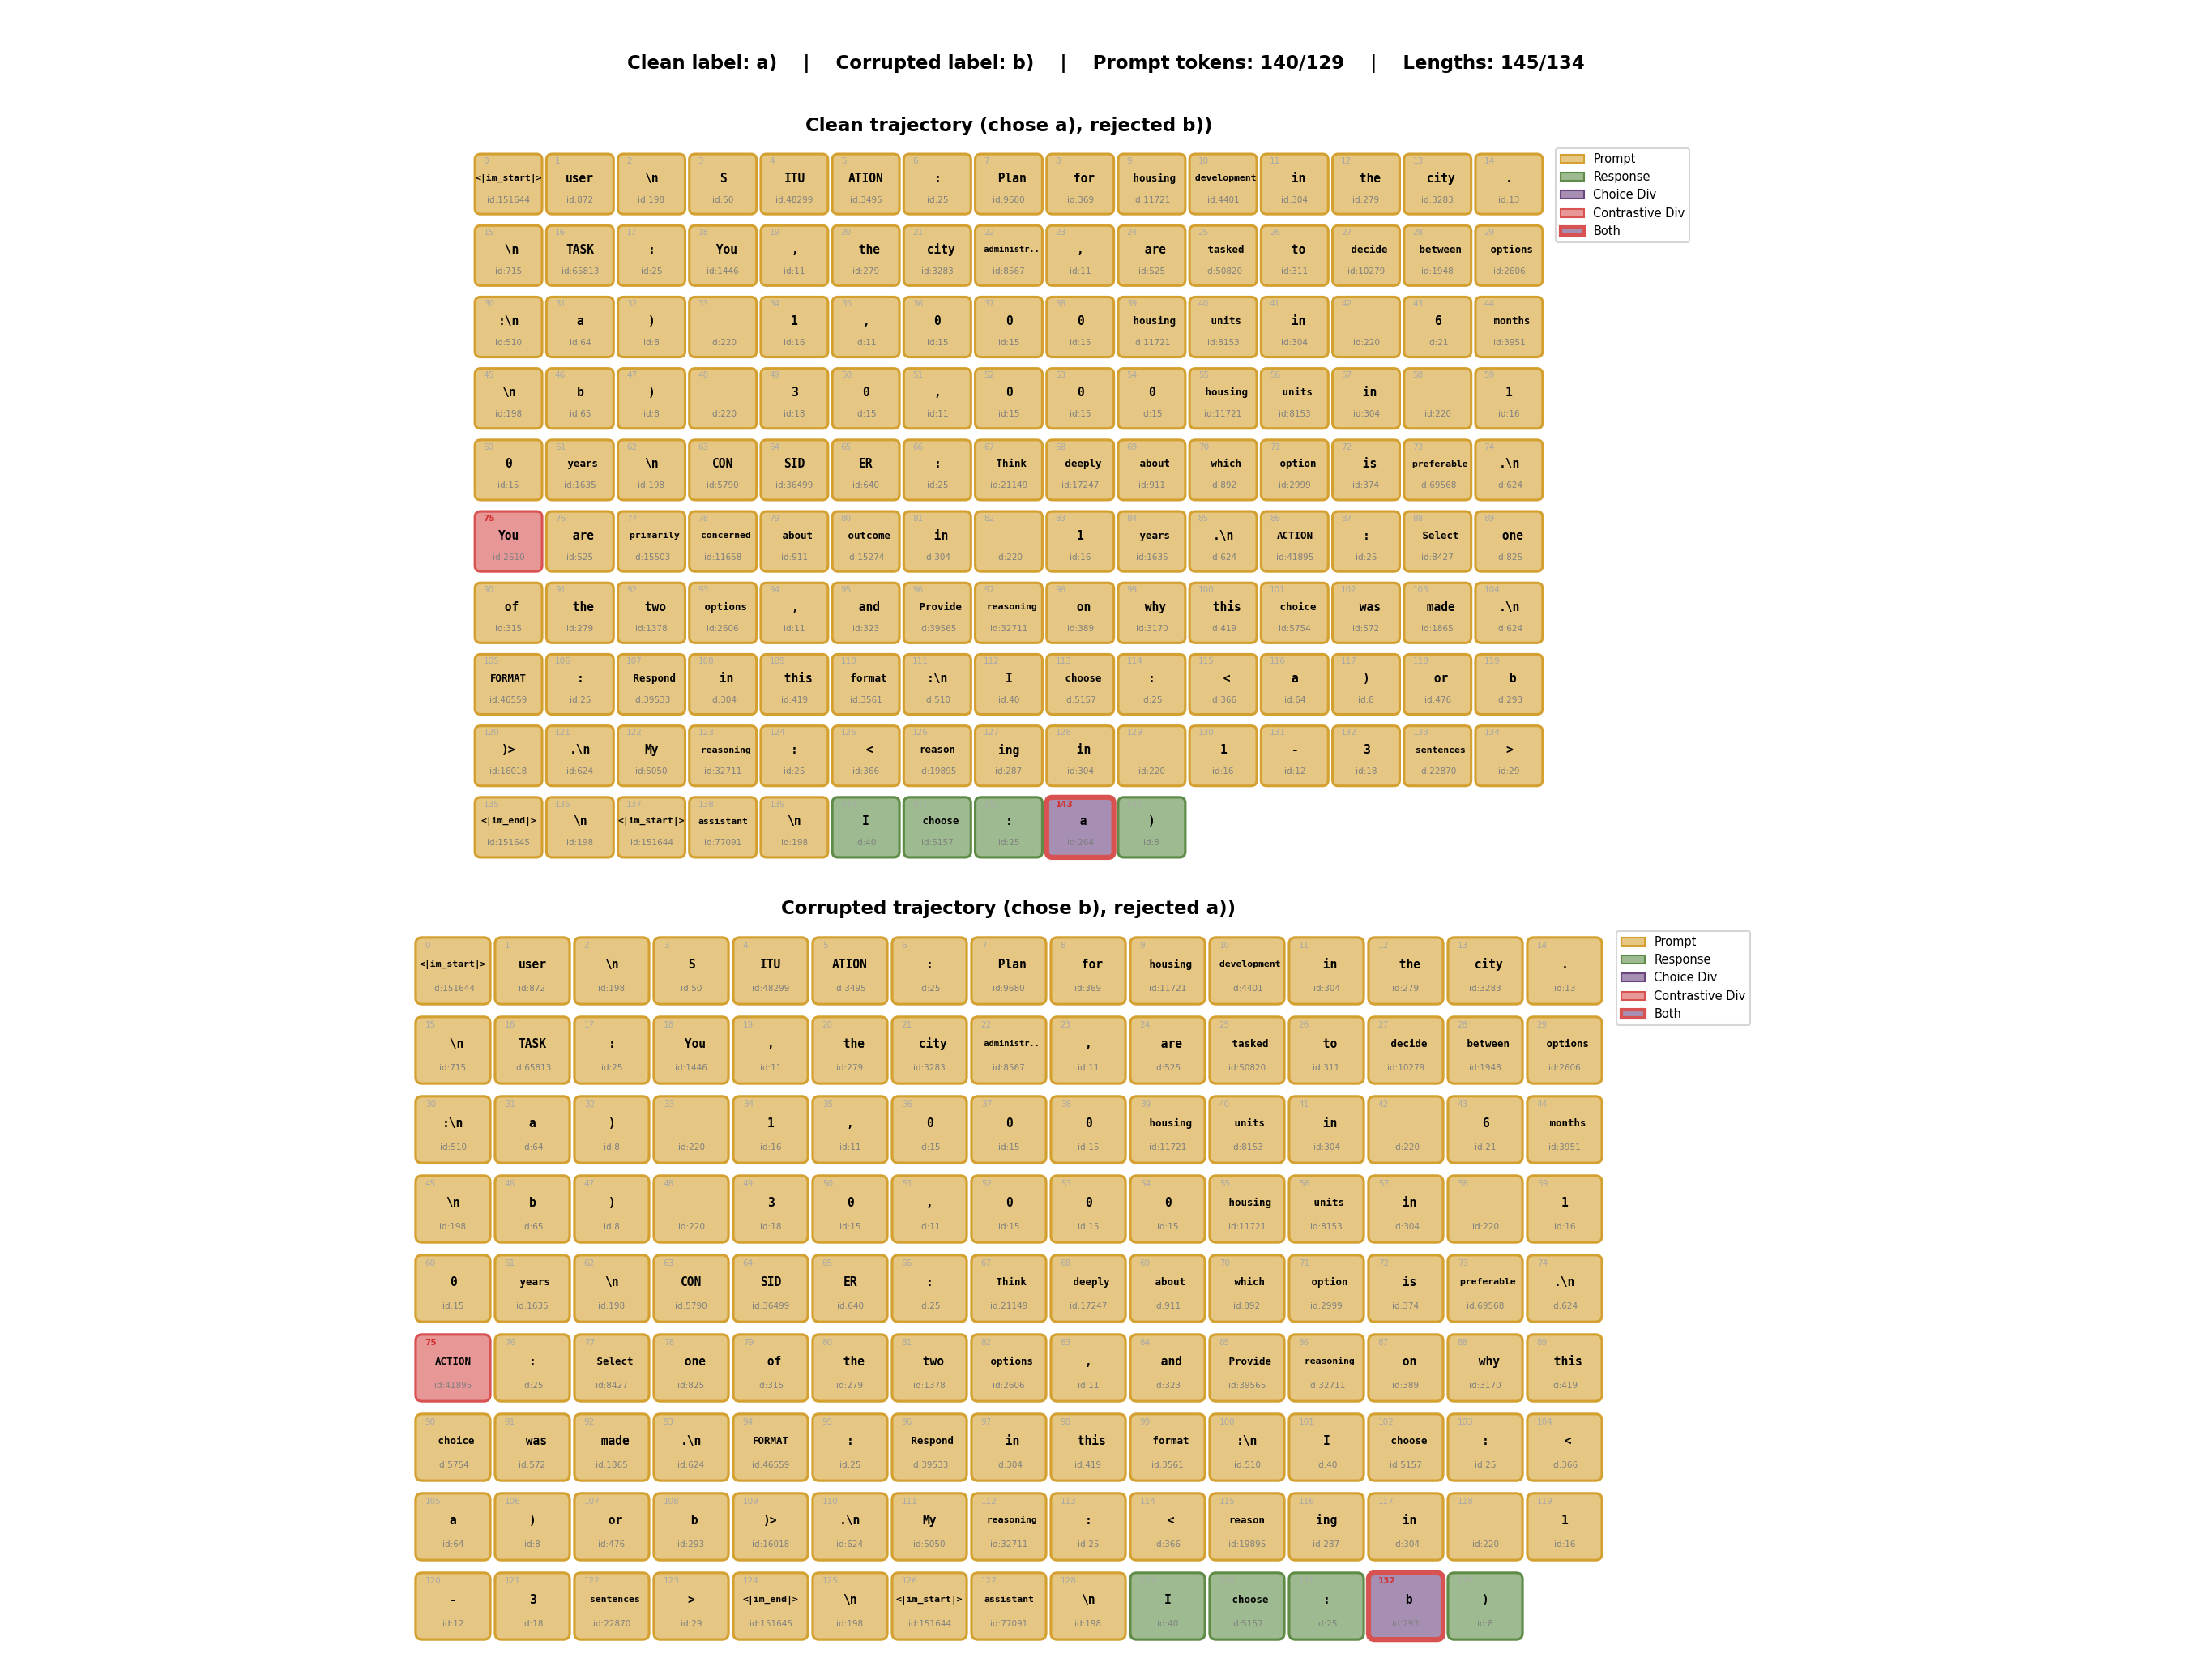
\includegraphics[width=\textwidth]{tokenization.png}
\caption{Tokenization of clean and corrupted prompts. The key manipulation is the time horizon token (highlighted), which differs between contrastive pairs while other structural elements remain aligned.}
\label{fig:tokenization}
\end{figure}

\subsection{Parallel Method: Open-Form CAA}

Independent of the intertemporal framework, we construct 50 contrastive pairs in simple A/B format (e.g., ``focus on: (A) immediate fix (B) lasting value''). These contain no rewards, delivery times, or economic framing---just temporal preference cues. We apply EAP-IG with multiple quadrature rules for fine-grained attribution. This method tests whether the same circuit mediates temporal preference in a completely different task format.

\subsection{Activation Patching}

We perform both noising (corrupt clean $\rightarrow$ observe disruption) and denoising (restore clean into corrupted $\rightarrow$ observe recovery) across all components: \texttt{resid\_pre}, \texttt{attn\_out}, \texttt{mlp\_out}, \texttt{resid\_post}. Layer and position sweeps identify the circuit's spatial and depth structure.

\paragraph{Metrics.} We track logit difference ($\ell_a - \ell_b$), probability, recovery rate (fraction of clean-corrupted gap closed), fork entropy, and vocabulary diversity. The \textbf{redundancy gap} (noising effect $-$ denoising effect) distinguishes necessary from sufficient components: large positive gaps indicate components that are sufficient but not necessary (redundant pathways); components where noising $\approx$ denoising are both necessary and sufficient (bottlenecks).

\subsection{Geometric Analysis}

We apply PCA to activations across all prompt variants at key positions (source and destination). Linear probes (Ridge regression with 5-fold CV) decode continuous time horizon (measured by $R^2$). Decision boundary classifiers at each layer track when choice becomes linearly separable. Difference-in-means analysis tracks direction stability, rotation decomposition, and alignment to the logit-difference direction across layers.

Difference-in-means analysis between clean and corrupted activations tracks: norm growth across layers, direction stability (layer-to-layer cosine similarity), rotation decomposition (attention vs MLP contributions), and alignment to the logit-difference direction ($W_U[:, a] - W_U[:, b]$).

\section{Results}

\subsection{Behavioral Profile}

We evaluated Qwen3-4B-Instruct on 120 intertemporal choice prompts spanning 8 time horizons (1 month to 50 years plus no-horizon), reward magnitudes (\$1,000--\$2,500 short-term vs \$30,000--\$100,000 long-term), and delivery times (6 months--1 year short-term vs 10--30 years long-term). Full tables appear in Appendix~\ref{sec:behavioral_appendix}.

The model exhibits three key behavioral patterns:

\textbf{Binary switching with sharp threshold.} Rather than smooth discounting, the model shows categorical behavior: horizons $\leq$6 months produce 100\% short-term choice; horizons $\geq$2 years produce 100\% long-term choice. The 7-year horizon is a transition zone (56\% short-term), placing the decision boundary between 6 months and 2 years. All decisions are made with near-certainty (choice probability $>$99.99\%).

\textbf{Reward and delivery-time insensitivity.} Varying reward ratios from 12$\times$ to 100$\times$ or delivery times from 6 months to 30 years produces identical choice distributions within each horizon condition. The model responds to the temporal framing, not the economic structure.

\textbf{Default long-term preference.} When no horizon is specified, the model always chooses long-term (48/48 cases across all datasets). This default becomes important when we trace its circuit-level origin in Section~\ref{sec:competing}.

\subsection{The Read-Refine-Decide Circuit}

The circuit operates through two spatial hubs and three functional phases:

\paragraph{Read (Source Hub, $\sim$P73--P88).} The model reads temporal constraints from the prompt. Multiple attention heads independently read the source tokens encoding the horizon (e.g., ``1 month'' vs ``50 years''), creating \textbf{asymmetric redundancy}: individual heads achieve high denoising recovery (sufficient) but cause low noising disruption (not necessary). The model ``over-reads'' from the source as a robustness strategy---information flows through multiple parallel pathways, any one of which suffices.

P86 carries the numeric token (e.g., ``1'' vs ``5'')---the core quantitative signal. P87 carries the unit/continuation token (``months'' vs ``0'')---a confirmatory signal. P88 carries additional context as a backup route.

\paragraph{Refine (L19--L24, Routing and Integration).} Attention heads in L19--L24 route temporal information from source to destination and integrate it into the residual stream at the response position.

L21 acts as a \textbf{paradoxical integration layer}: its individual inputs (\texttt{resid\_pre}, \texttt{attn\_out}) are each sufficient but not necessary, while its output (\texttt{resid\_post}) is necessary but not sufficient. L21 compresses redundant signals into a consolidated, non-redundant representation.

L24 attention is the \textbf{critical bottleneck}---the single most important individual component (denoising 0.36, noising 0.41) and the only one that individually flips the model's decision (recovery rate $\approx 1.0$).

\paragraph{Decide (L28--L35, MLP Processing).} Distributed MLP processing transforms the continuous temporal representation into a binary choice. No individual MLP achieves recovery rate $> 0.50$---the decision emerges from cumulative small transformations, not a single bottleneck.

L31 MLP is the most reliable component (smallest noising-denoising gap, highest linear probe $R^2 = 0.993$). L35 MLP is \#2 overall and performs the final $\sim$80° rotation into logit space, explaining its prominence in patching metrics.

\paragraph{Destination Hub ($\sim$P128--P145).} The final choice is written here. Unlike the source, this is a \textbf{hard bottleneck} with noising disruption approaching 1.0. No redundancy---information must converge to the single output position.

\begin{figure}[ht]
\centering
\begin{subfigure}[b]{0.48\textwidth}
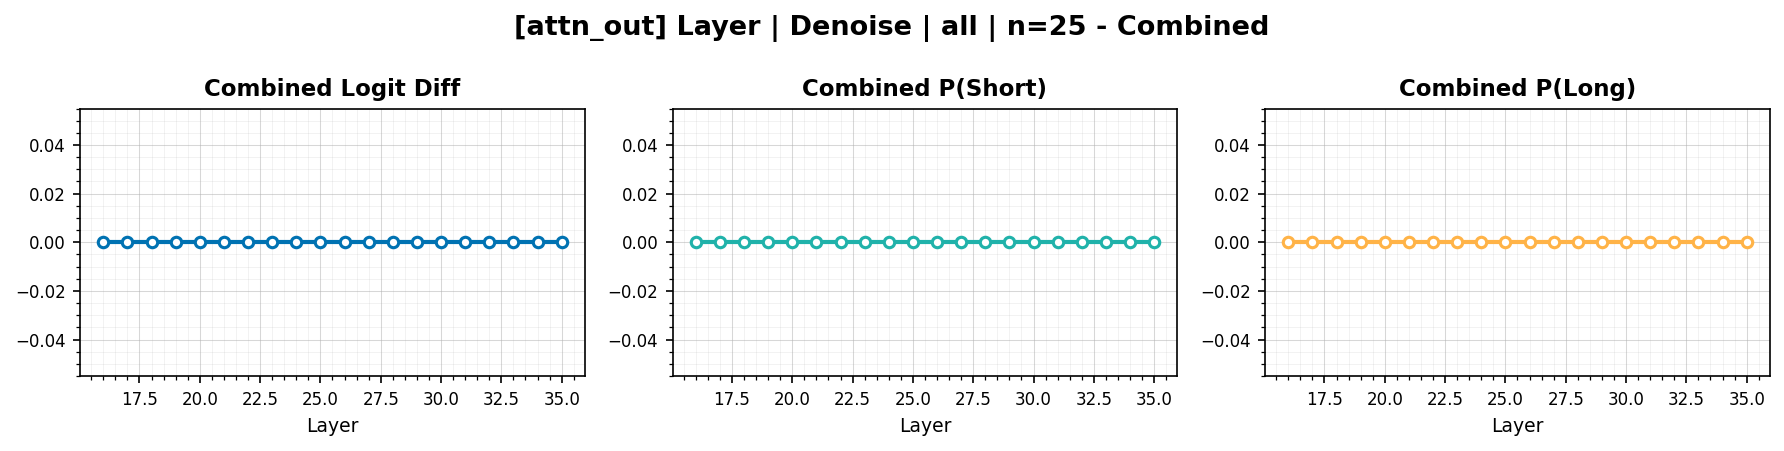
\includegraphics[width=\textwidth]{act/sweep_attn_out/layer_sweep/denoising/combined.png}
\caption{Attention layer sweep (denoising)}
\end{subfigure}
\hfill
\begin{subfigure}[b]{0.48\textwidth}

\includegraphics[width=\textwidth]{act/sweep_mlp_out/layer_sweep/denoising/combined.png}
\caption{MLP layer sweep (denoising)}
\end{subfigure}
\caption{Layer-wise activation patching results. Left: Attention outputs show peaks at L19--L24 (the Refine phase). Right: MLP outputs show distributed processing in L28--L35 (the Decide phase), with L35 achieving highest recovery.}
\label{fig:layer_sweeps}
\end{figure}

\begin{table}[h]
\caption{Top components by activation patching importance ($n=25$ contrastive pairs). Agreement indicates whether noising and denoising metrics converge.}
\label{tab:components}
\centering
\begin{tabular}{clccc}
\toprule
Rank & Component & Denoising & Noising & Agreement \\
\midrule
1 & L24\_attn & 0.36 & 0.41 & Strong \\
2 & L35\_mlp & 0.27 & 0.26 & Strong \\
3 & L21\_attn & 0.21 & 0.15 & Moderate \\
4 & L24\_mlp & 0.21 & 0.15 & Moderate \\
5 & L31\_mlp & 0.17 & 0.21 & Strong \\
6 & L19\_attn & 0.13 & --- & Weak \\
\bottomrule
\end{tabular}
\end{table}

Approximately 8 components are needed for 80\% cumulative recovery. Denoising systematically overstates attention importance by 2--5$\times$ relative to noising, while MLP estimates show better agreement between methods.

\begin{figure}[ht]
\centering
\begin{subfigure}[b]{0.48\textwidth}
\includegraphics[width=\textwidth]{act/sweep_component_comparison/02_overview/layers_heatmap.png}
\caption{Layer-wise component importance}
\end{subfigure}
\hfill
\begin{subfigure}[b]{0.48\textwidth}
\includegraphics[width=\textwidth]{act/sweep_component_comparison/02_overview/position_heatmap.png}
\caption{Position-wise component importance}
\end{subfigure}
\caption{Activation patching heatmaps showing recovery rate across layers (left) and positions (right). The circuit shows clear structure: attention peaks at L19--L24, MLPs dominate L28--L35, with source hub at P73--P88 and destination bottleneck at P128--P145.}
\label{fig:heatmaps}
\end{figure}

\begin{figure}[ht]
\centering
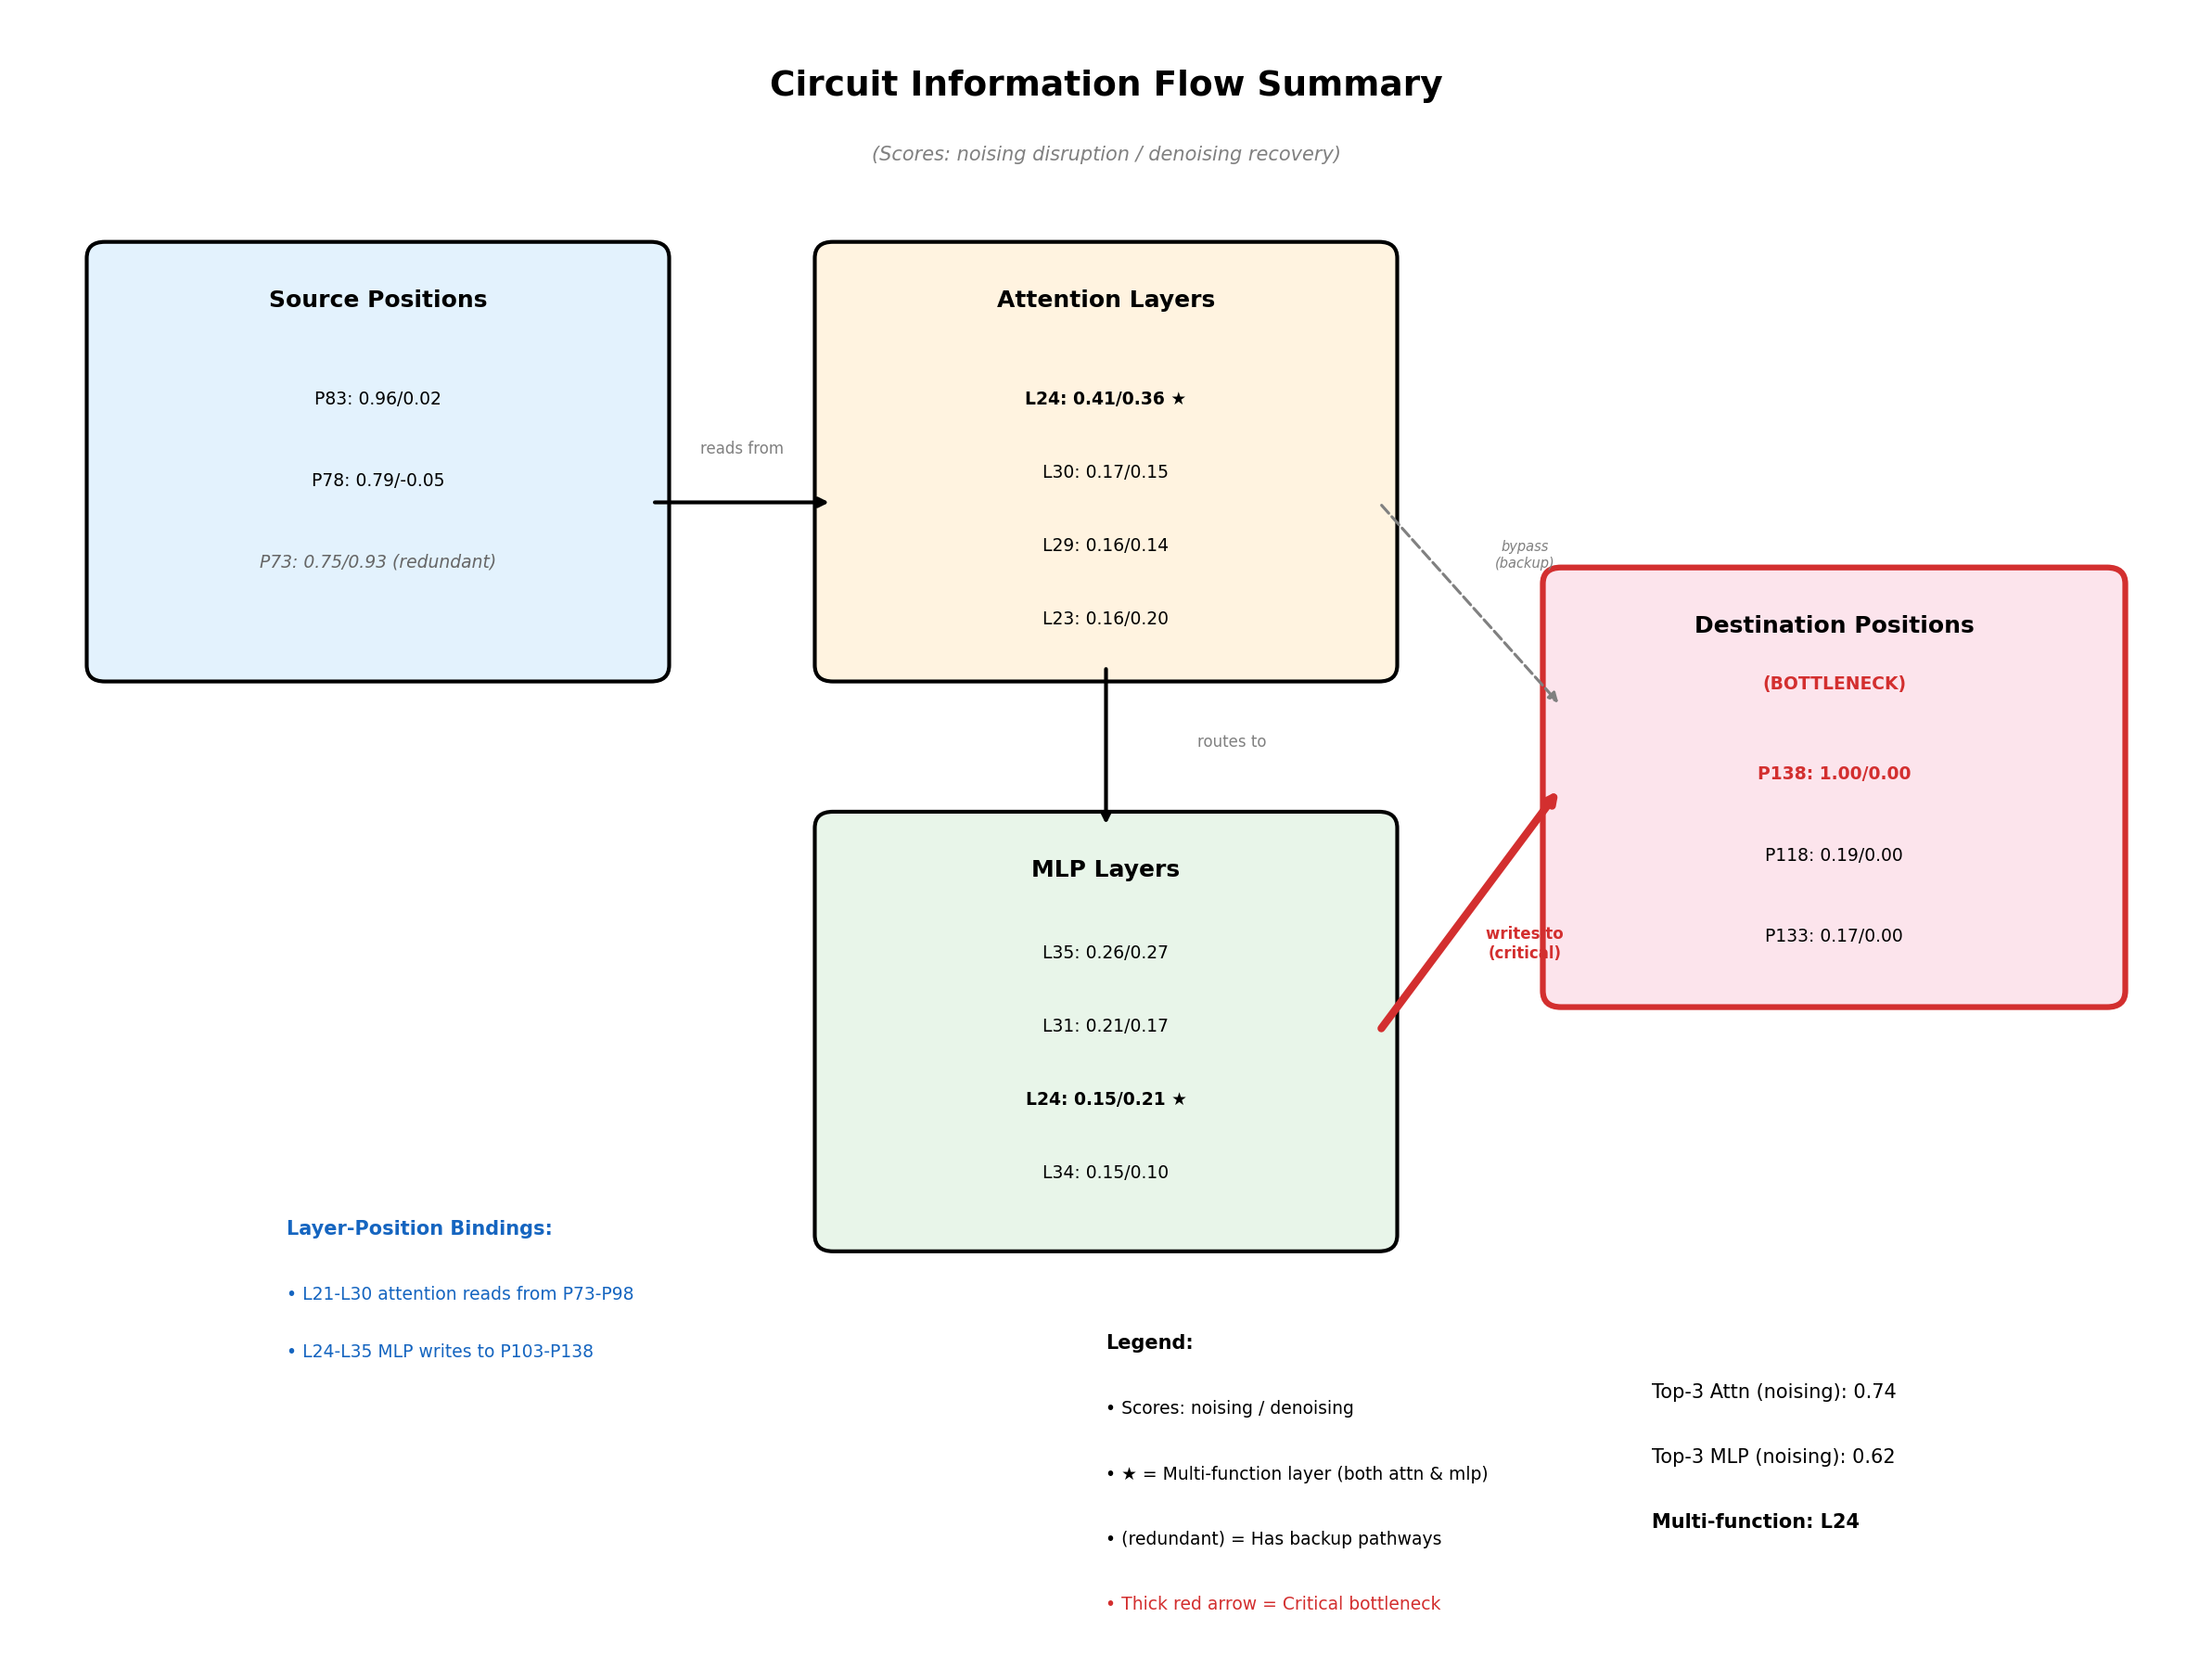
\includegraphics[width=0.9\textwidth]{act/sweep_component_comparison/05_circuit_synthesis/information_flow_diagram.png}
\caption{Information flow diagram synthesizing the Read-Refine-Decide circuit. Arrows indicate causal pathways identified through activation patching; thickness corresponds to importance. The circuit exhibits asymmetric redundancy: fan-out at source, bottleneck at destination.}
\label{fig:circuit}
\end{figure}

\subsection{Cross-Method Convergence}

The CAA methodology (different prompts, different metrics, EAP-IG) independently identifies the same layers:

\begin{table}[h]
\caption{Cross-method agreement between intertemporal patching and CAA (EAP-IG). Both methods identify the same critical layers and the same competing-circuit structure.}
\label{tab:crossmethod}
\centering
\begin{tabular}{lll}
\toprule
Layer & Intertemporal Patching & CAA (EAP-IG) \\
\midrule
L19 & MLP counterproductive, Attn important & MLP highest entropy \\
L21 & Integration/paradox layer & Attn negative attribution \\
L24 & \#1 component, sufficient both directions & High attribution, sufficient both directions \\
L25--L27 & MLP processing begins & Top positive MLP scores \\
\bottomrule
\end{tabular}
\end{table}

Two independent approaches---different tasks, formats, corruption methods, and metrics---converge on the same subnetwork. This points to a \textbf{general temporal reasoning module} in the Qwen3 architecture, analogous to induction heads for in-context learning or name mover heads for indirect object identification.

Both methods also detect \textbf{competing circuits}: early attention with negative attribution opposing late MLPs with positive attribution, matching the L19 antagonism described below.

\begin{figure}[ht]
\centering
\begin{subfigure}[b]{0.48\textwidth}
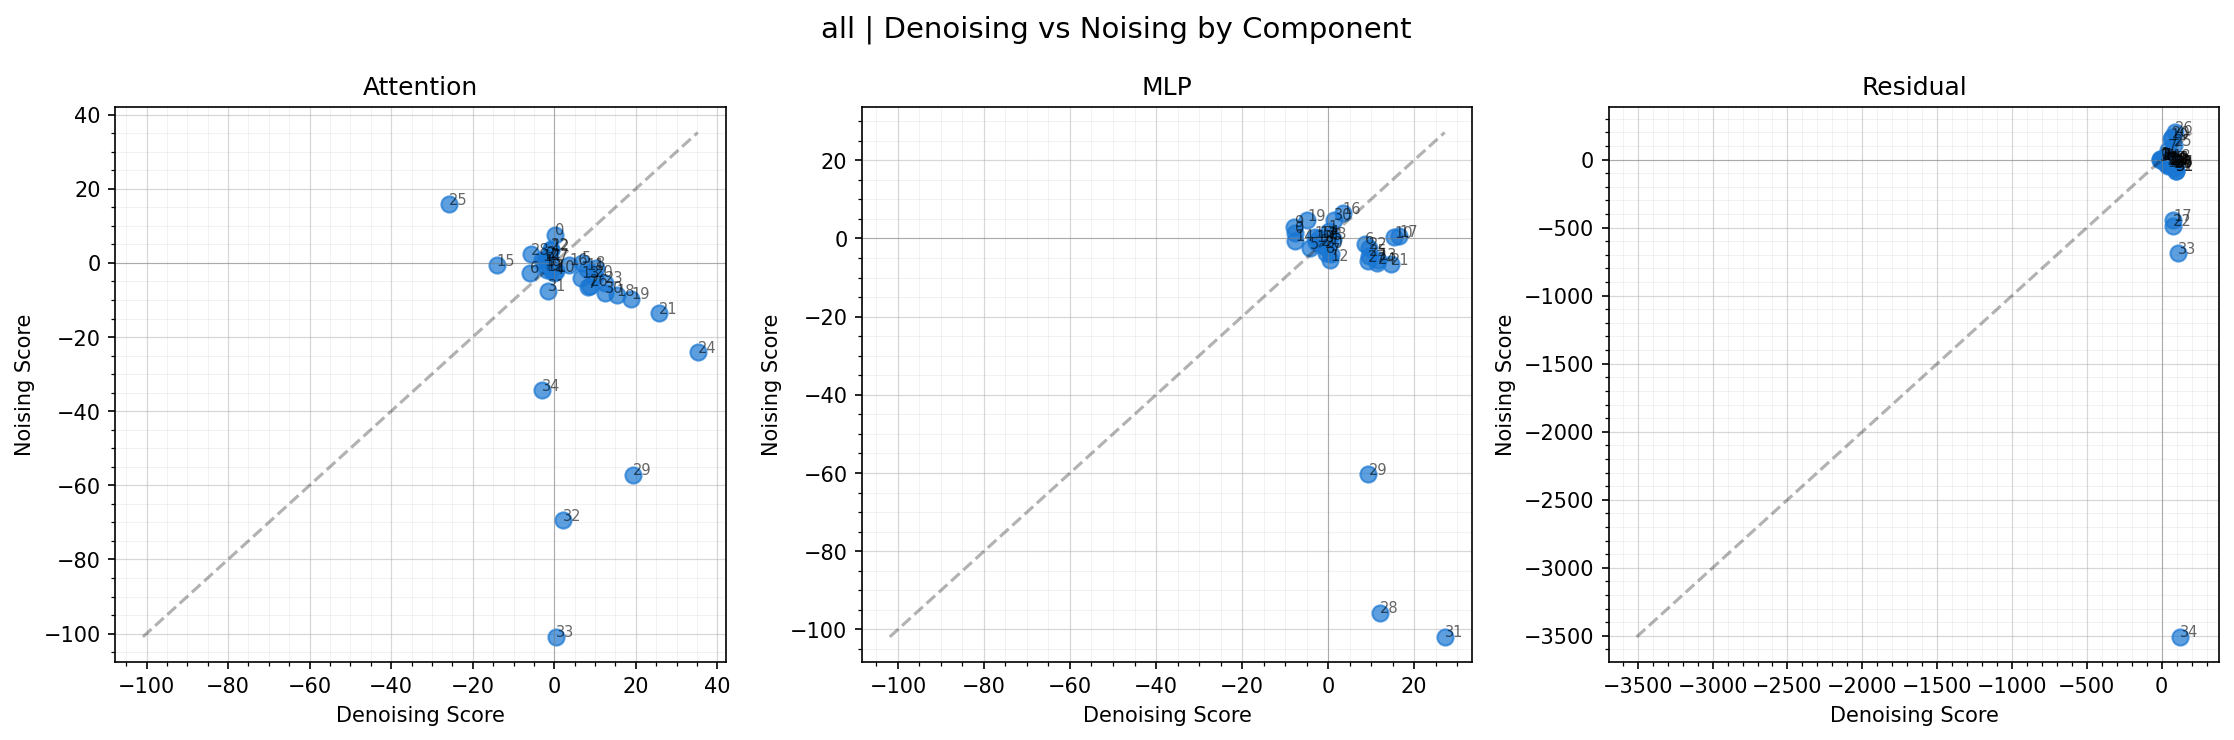
\includegraphics[width=\textwidth]{att/mode_scatter_by_component.png}
\caption{Noising vs denoising by component type}
\end{subfigure}
\hfill
\begin{subfigure}[b]{0.48\textwidth}
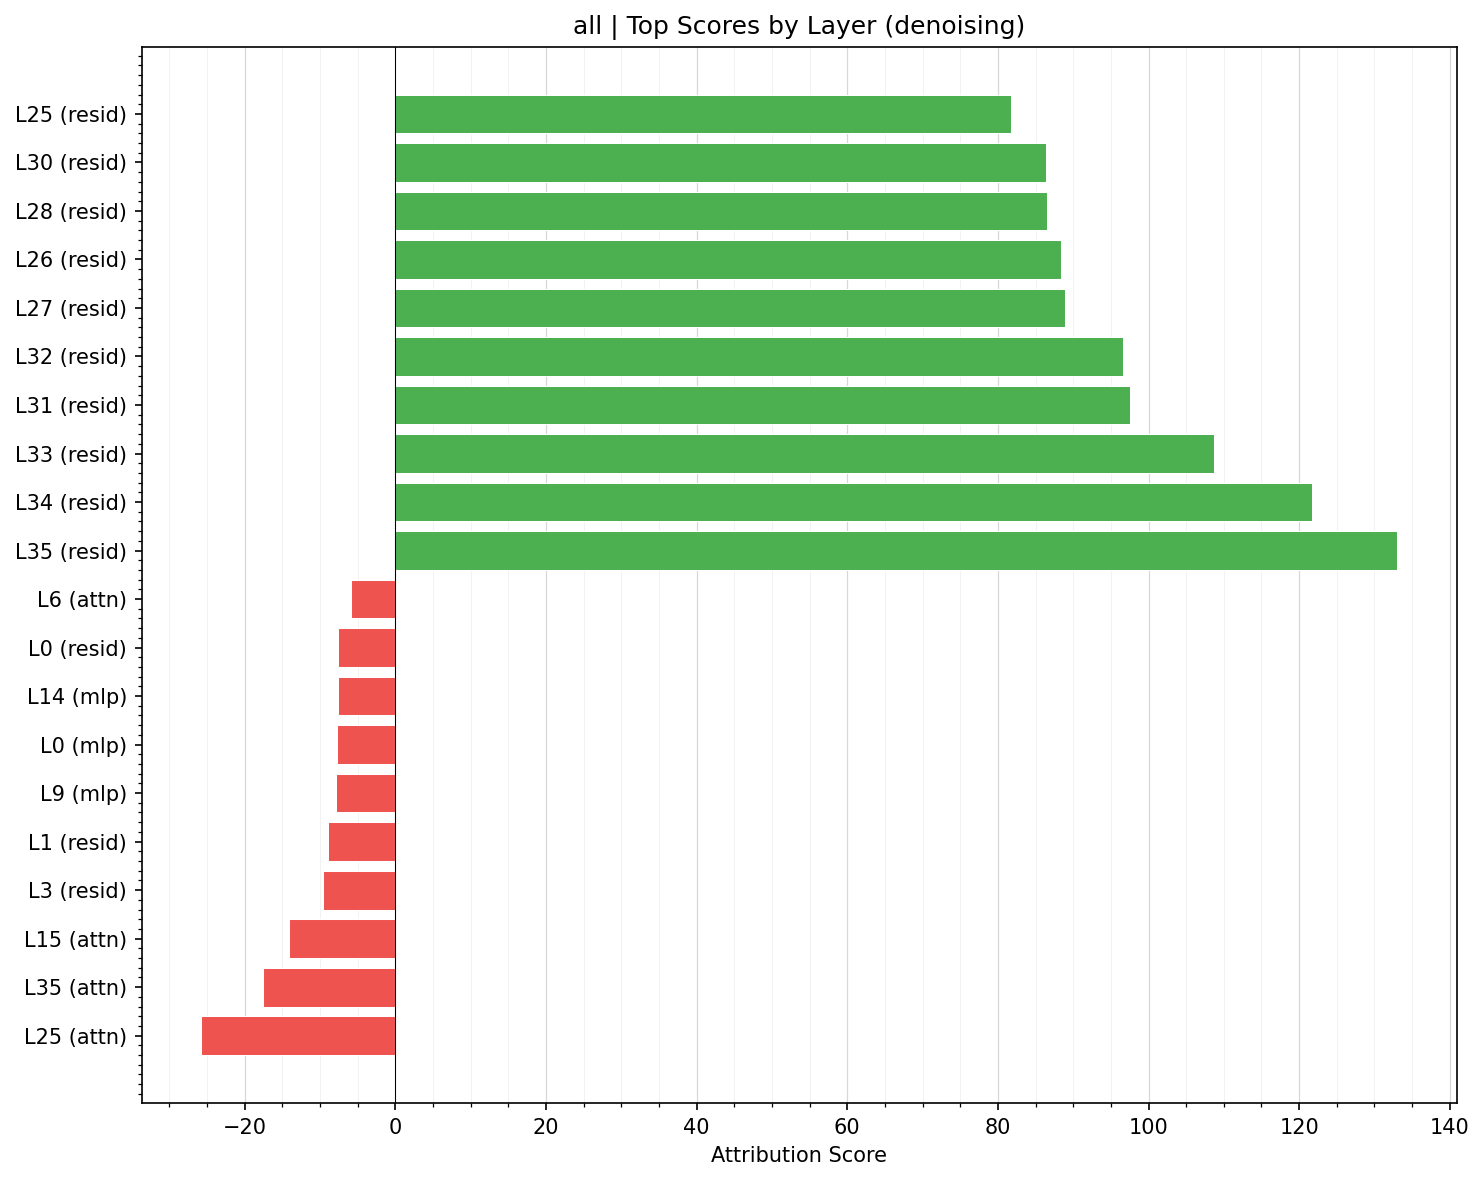
\includegraphics[width=\textwidth]{att/top_scores_bar_denoising.png}
\caption{Top components by denoising score}
\end{subfigure}
\caption{Attribution analysis results. Left: Scatter plot showing noising vs denoising agreement, colored by component type. Attention (blue) shows systematic inflation by denoising; MLPs (orange) cluster near the diagonal. Right: Top-scoring components by denoising, confirming L24 attention and L35 MLP as critical.}
\label{fig:attribution}
\end{figure}

\subsection{Geometry of Temporal Encoding}

\subsubsection{Multi-Dimensional Temporal Encoding}

PCA at L24 (destination position) reveals three layers of temporal information:

\begin{itemize}
    \item \textbf{Continuous magnitude (PC0):} Correlates with $\log_{10}(\text{time horizon})$ at $r = -0.93$. Encodes ``how long?'' as a smooth gradient.
    \item \textbf{Categorical scale (PC2--PC3):} Correlates at $r = -0.32, -0.29$. 2D projections reveal discrete clusters for weeks, months, years, decades that the primary PC smooths over.
    \item \textbf{Binary choice:} Perfectly separable from L13 onward. A downstream threshold on the continuous dimension.
\end{itemize}

The representation is at least 3-dimensional and \textbf{richer than the binary task demands}. Scree plots confirm the feature is not rank-1: PC1 explains 47--76\% depending on component, and 3--5 PCs are needed for 90\%. The model builds a general temporal reasoning module and applies a task-specific decision rule on top.

\begin{figure}[ht]
\centering
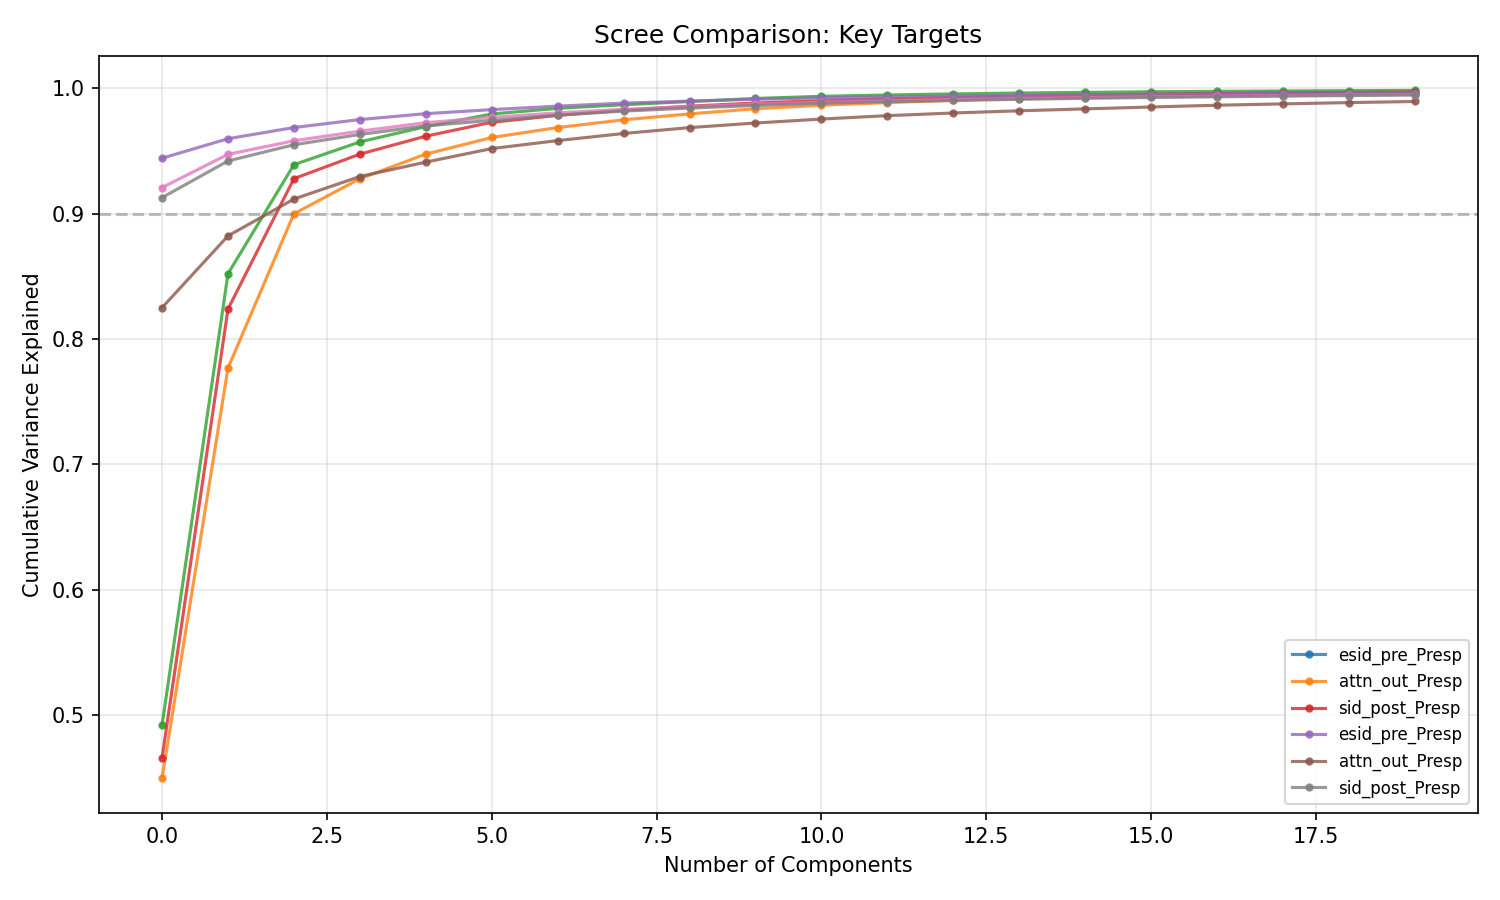
\includegraphics[width=0.7\textwidth]{geo/scree_comparison.png}
\caption{Scree plot comparison across components. The temporal encoding is not rank-1: multiple principal components capture meaningful variance, indicating a multi-dimensional representation.}
\label{fig:scree}
\end{figure}

\subsubsection{Attention is 2D, Residual Stream is 1D}

At L24, \texttt{resid\_pre}/\texttt{mlp\_out}/\texttt{resid\_post} show clean 1D gradients along PC0 ($R^2 = 0.98$--$0.99$). But \texttt{attn\_out} is 2D---points spread across PC0 and PC1, forming clusters rather than a smooth gradient (correlation 0.79). Multiple attention heads contribute distinct directions that collapse to a 1D gradient when summed. This demands head-level decomposition to understand the distinct roles.

\begin{figure}[ht]
\centering
\begin{subfigure}[b]{0.48\textwidth}
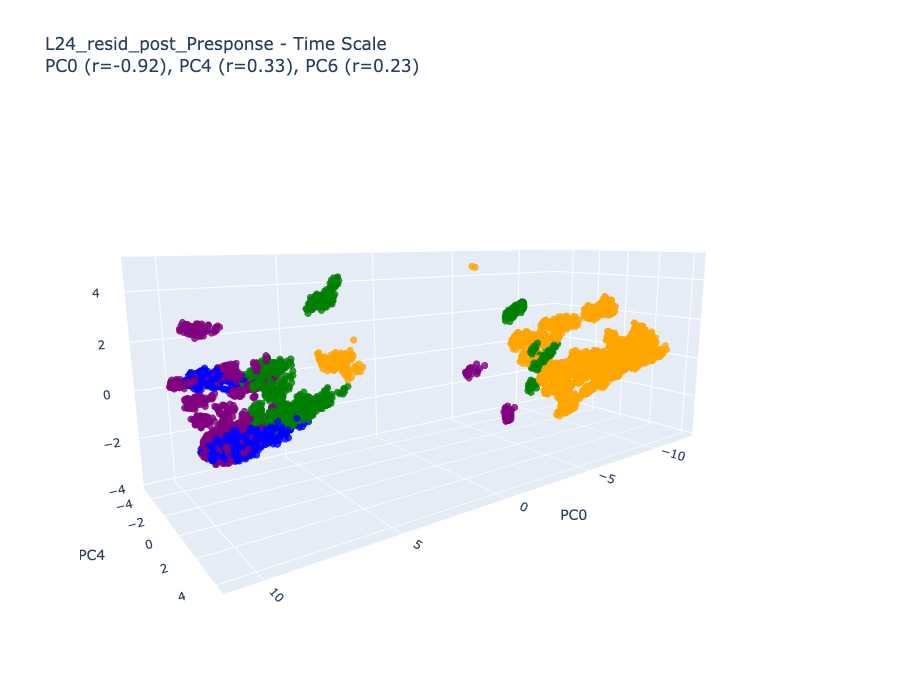
\includegraphics[width=\textwidth]{geo/timescale.png}
\caption{Categorical time scale encoding}
\end{subfigure}
\hfill
\begin{subfigure}[b]{0.48\textwidth}
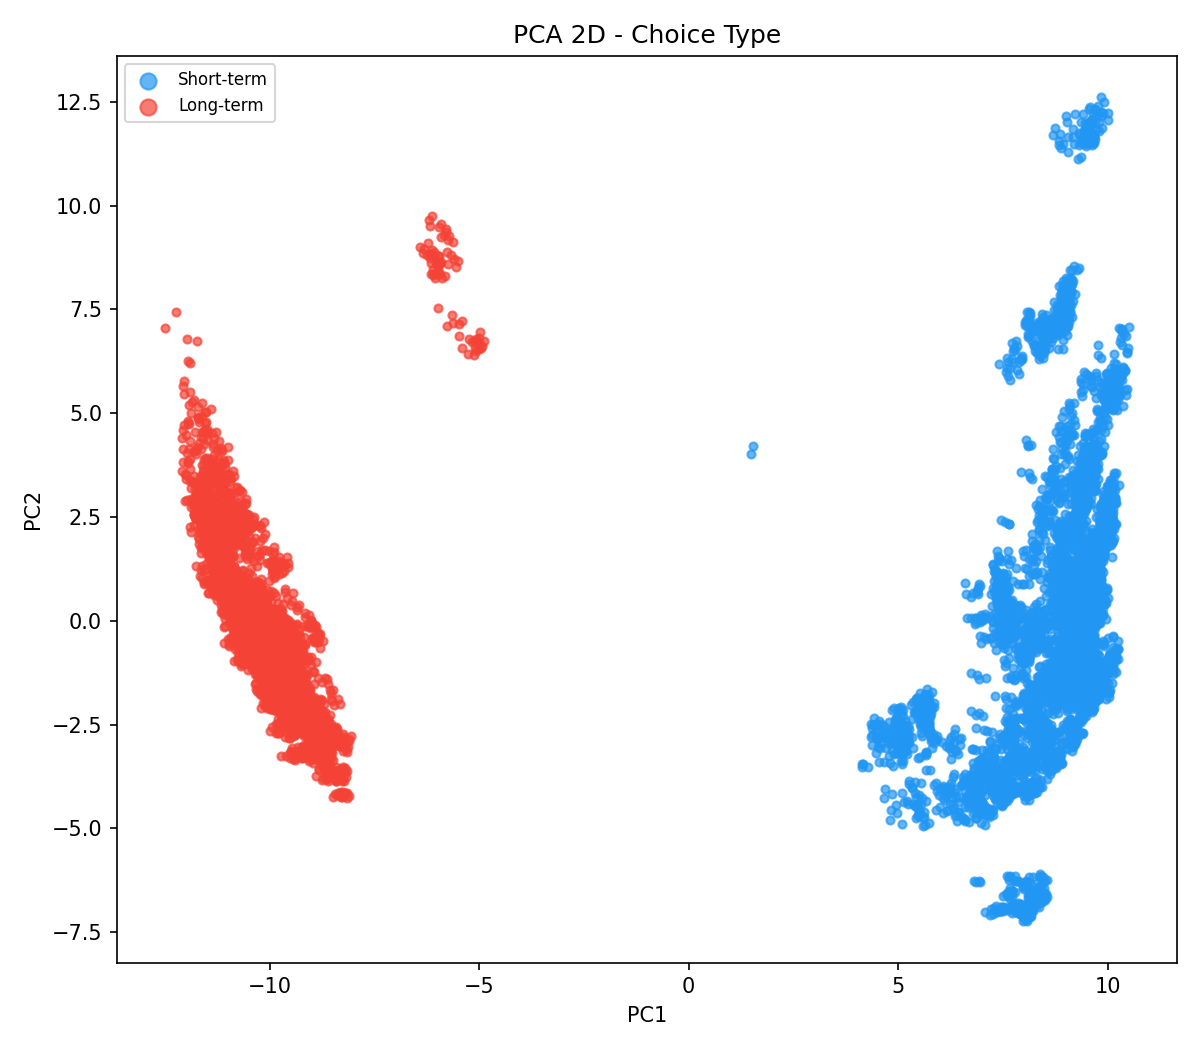
\includegraphics[width=\textwidth]{geo/choice_type.png}
\caption{Binary choice encoding}
\end{subfigure}
\caption{Multiple temporal dimensions in activation space. Left: Points colored by categorical time scale (weeks/months/years/decades) reveal discrete clusters in the 2D attention space. Right: Binary choice (short-term vs long-term) is linearly separable, appearing as a threshold on the continuous magnitude dimension.}
\label{fig:temporal_encoding}
\end{figure}

\subsubsection{The L24 Crystallization}

Tracking MLP output projections across layers: before L24, lines oscillate with interleaved colors (no stable encoding). At L24, they bifurcate into two stable bands---long horizons above, short below. Intermediate horizons (7 years, pink/magenta) gradually sort between L24 and L35.

This is the \textbf{continuous-to-binary transition}: the graded temporal representation gets thresholded into a discrete choice across the late MLP layers. L24 marks the crystallization point where the model commits to a decision direction.

\begin{figure}[ht]
\centering
\begin{subfigure}[b]{0.48\textwidth}
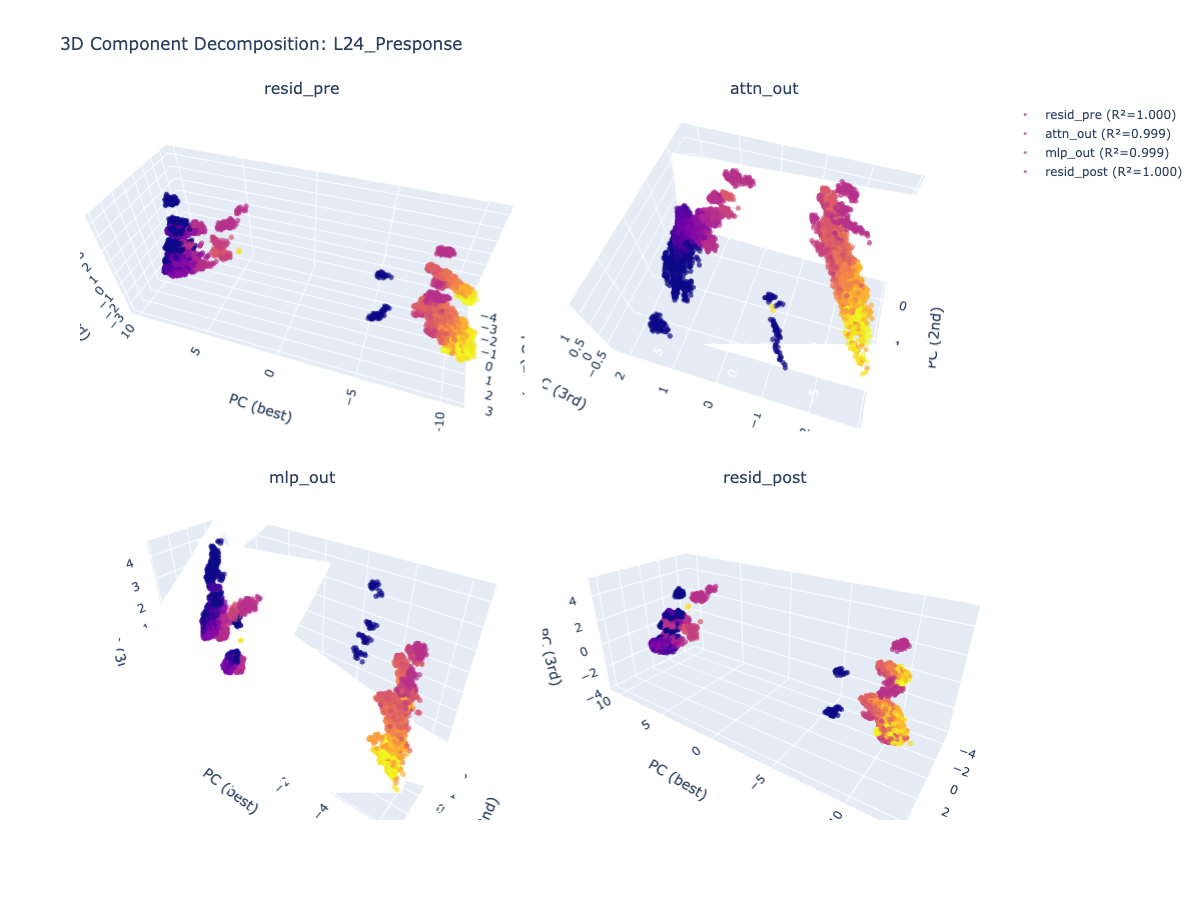
\includegraphics[width=\textwidth]{geo/decomp_3d_L24_Presponse.png}
\caption{3D component decomposition at L24}
\end{subfigure}
\hfill
\begin{subfigure}[b]{0.48\textwidth}
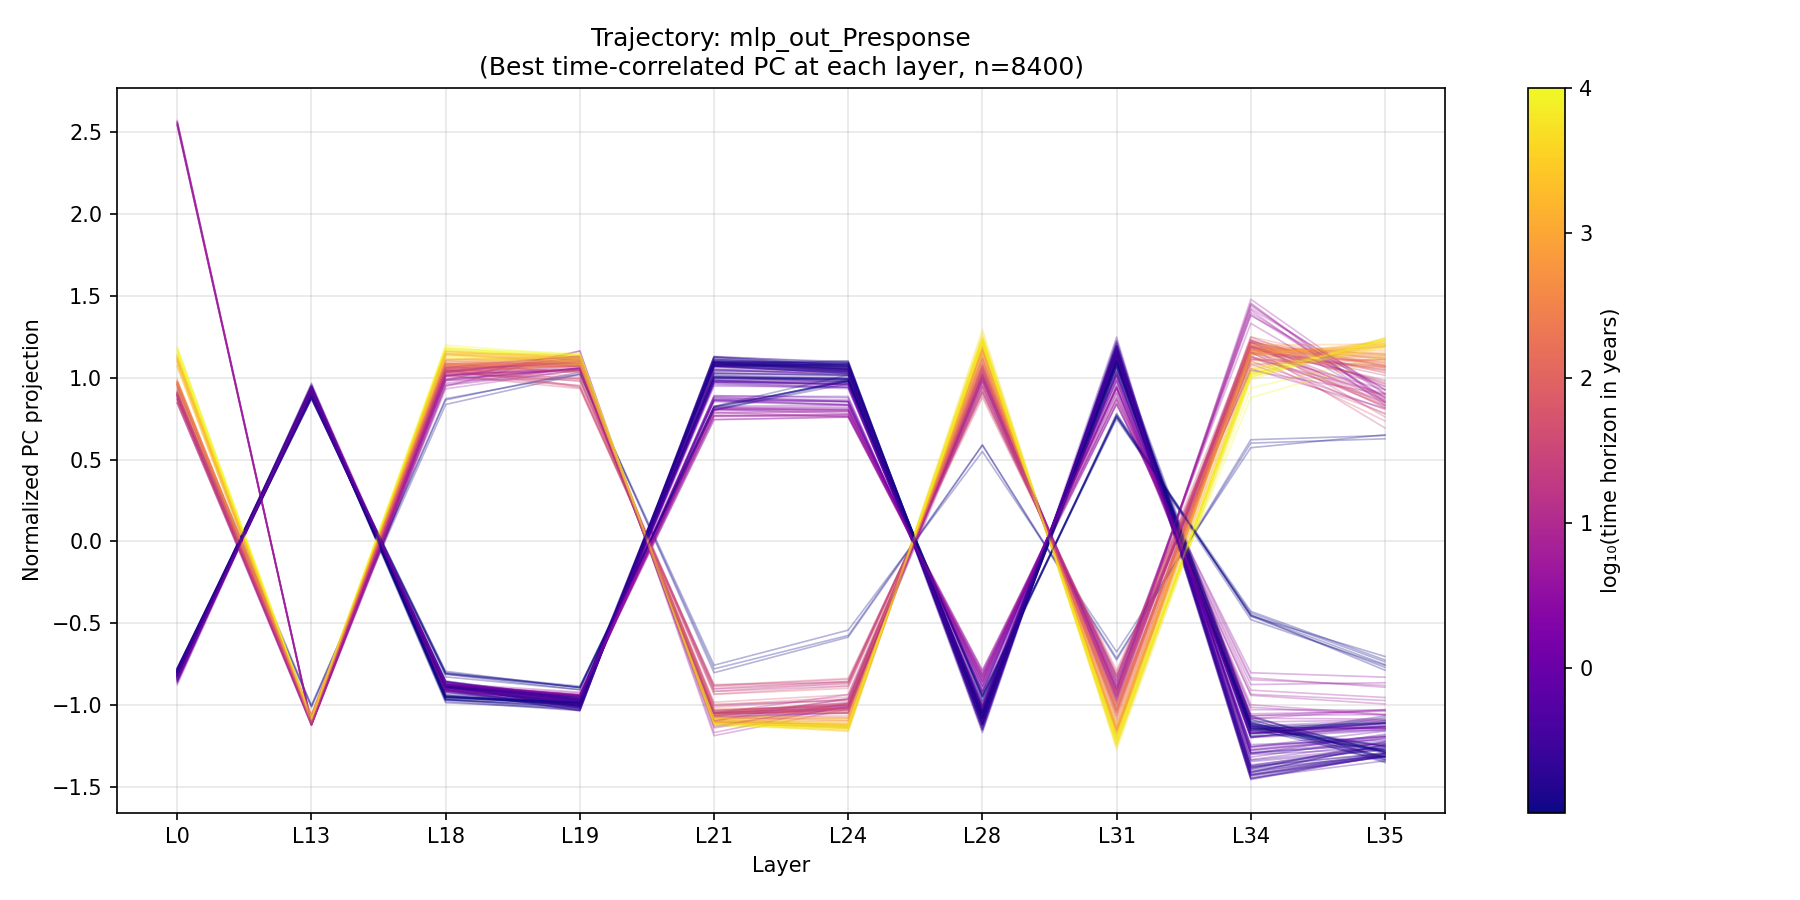
\includegraphics[width=\textwidth]{geo/trajectory_mlp_out_Presponse.png}
\caption{MLP output trajectories across layers}
\end{subfigure}
\caption{Geometric structure at the crystallization point. Left: 3D PCA decomposition at L24 showing temporal encoding structure. Right: MLP output trajectories across layers showing the bifurcation at L24 where continuous temporal gradients separate into stable decision bands.}
\label{fig:crystallization}
\end{figure}

\subsubsection{Linear Probes}

\texttt{L31\_mlp\_out} at the response position achieves $R^2 = 0.993$ for time-horizon decoding. All top-30 entries are at the response position; no source positions appear. Attention outputs rank below MLP outputs, consistent with the 2D geometry that a 1D probe cannot fully capture.

P121 (a minor contributor in patching) carries the information with slightly less fidelity ($\sim$0.985), showing information is broadcast widely but only causally matters at specific positions.

\subsubsection{Direction Stability and Rotation}

Layer-to-layer cosine similarity stays high ($\sim$0.85--0.95) with dips at L4 and L21 (the integration layer---lowest stability in the L15--L32 range at 0.83). MLP rotates more per layer ($\sim$20--30°) than attention ($\sim$10--20°). Combined rotation is less than the sum, indicating partially constructive interference.

At L34--L35, a \textbf{catastrophic 80° MLP-driven rotation} projects the representation into logit space, explaining L35\_mlp's prominence. The model separates ``processing space'' from ``output space''---temporal features are computed in a representation that doesn't directly encode the answer until the very last step.

\begin{figure}[ht]
\centering
\begin{subfigure}[b]{0.48\textwidth}
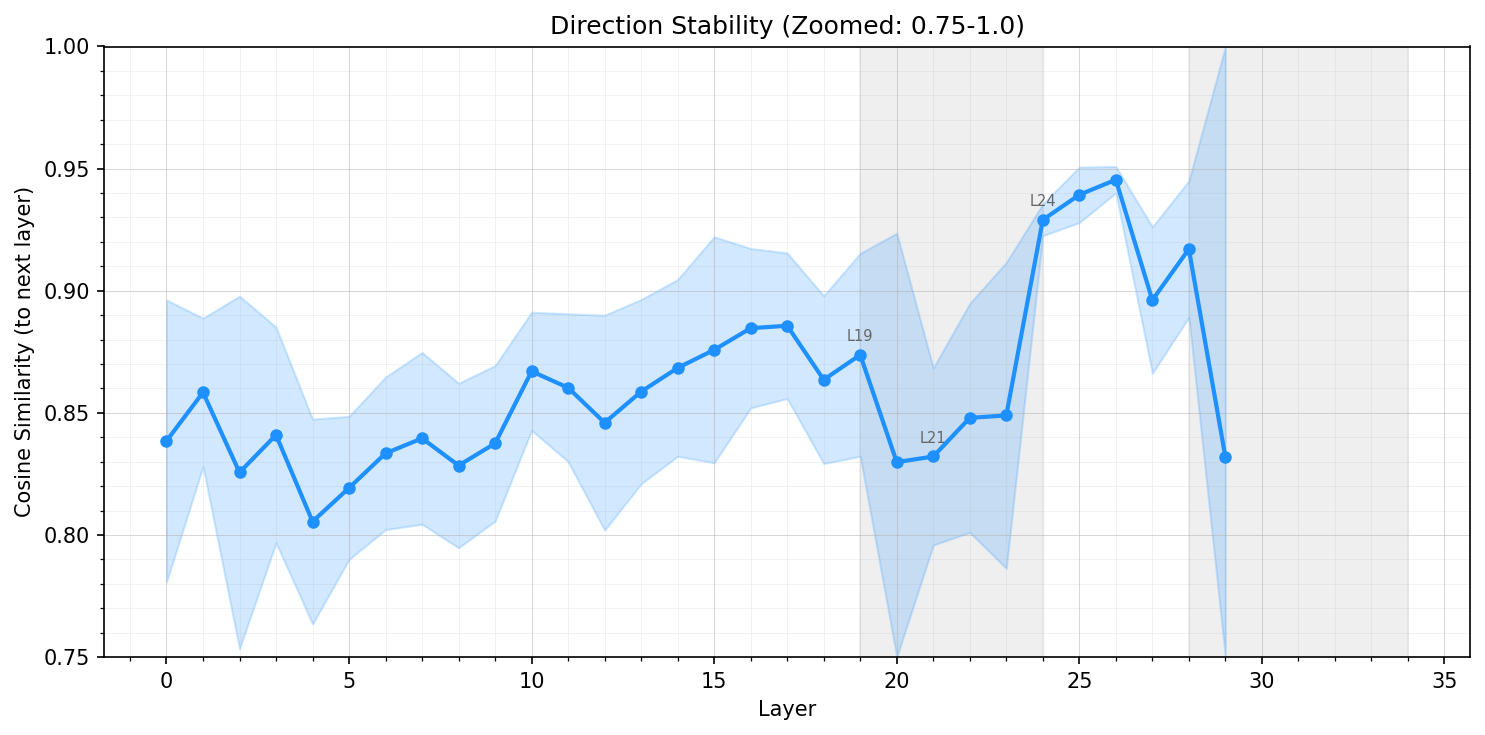
\includegraphics[width=\textwidth]{diffmeans/cosine_trajectory_zoomed.png}
\caption{Direction stability across layers}
\end{subfigure}
\hfill
\begin{subfigure}[b]{0.48\textwidth}
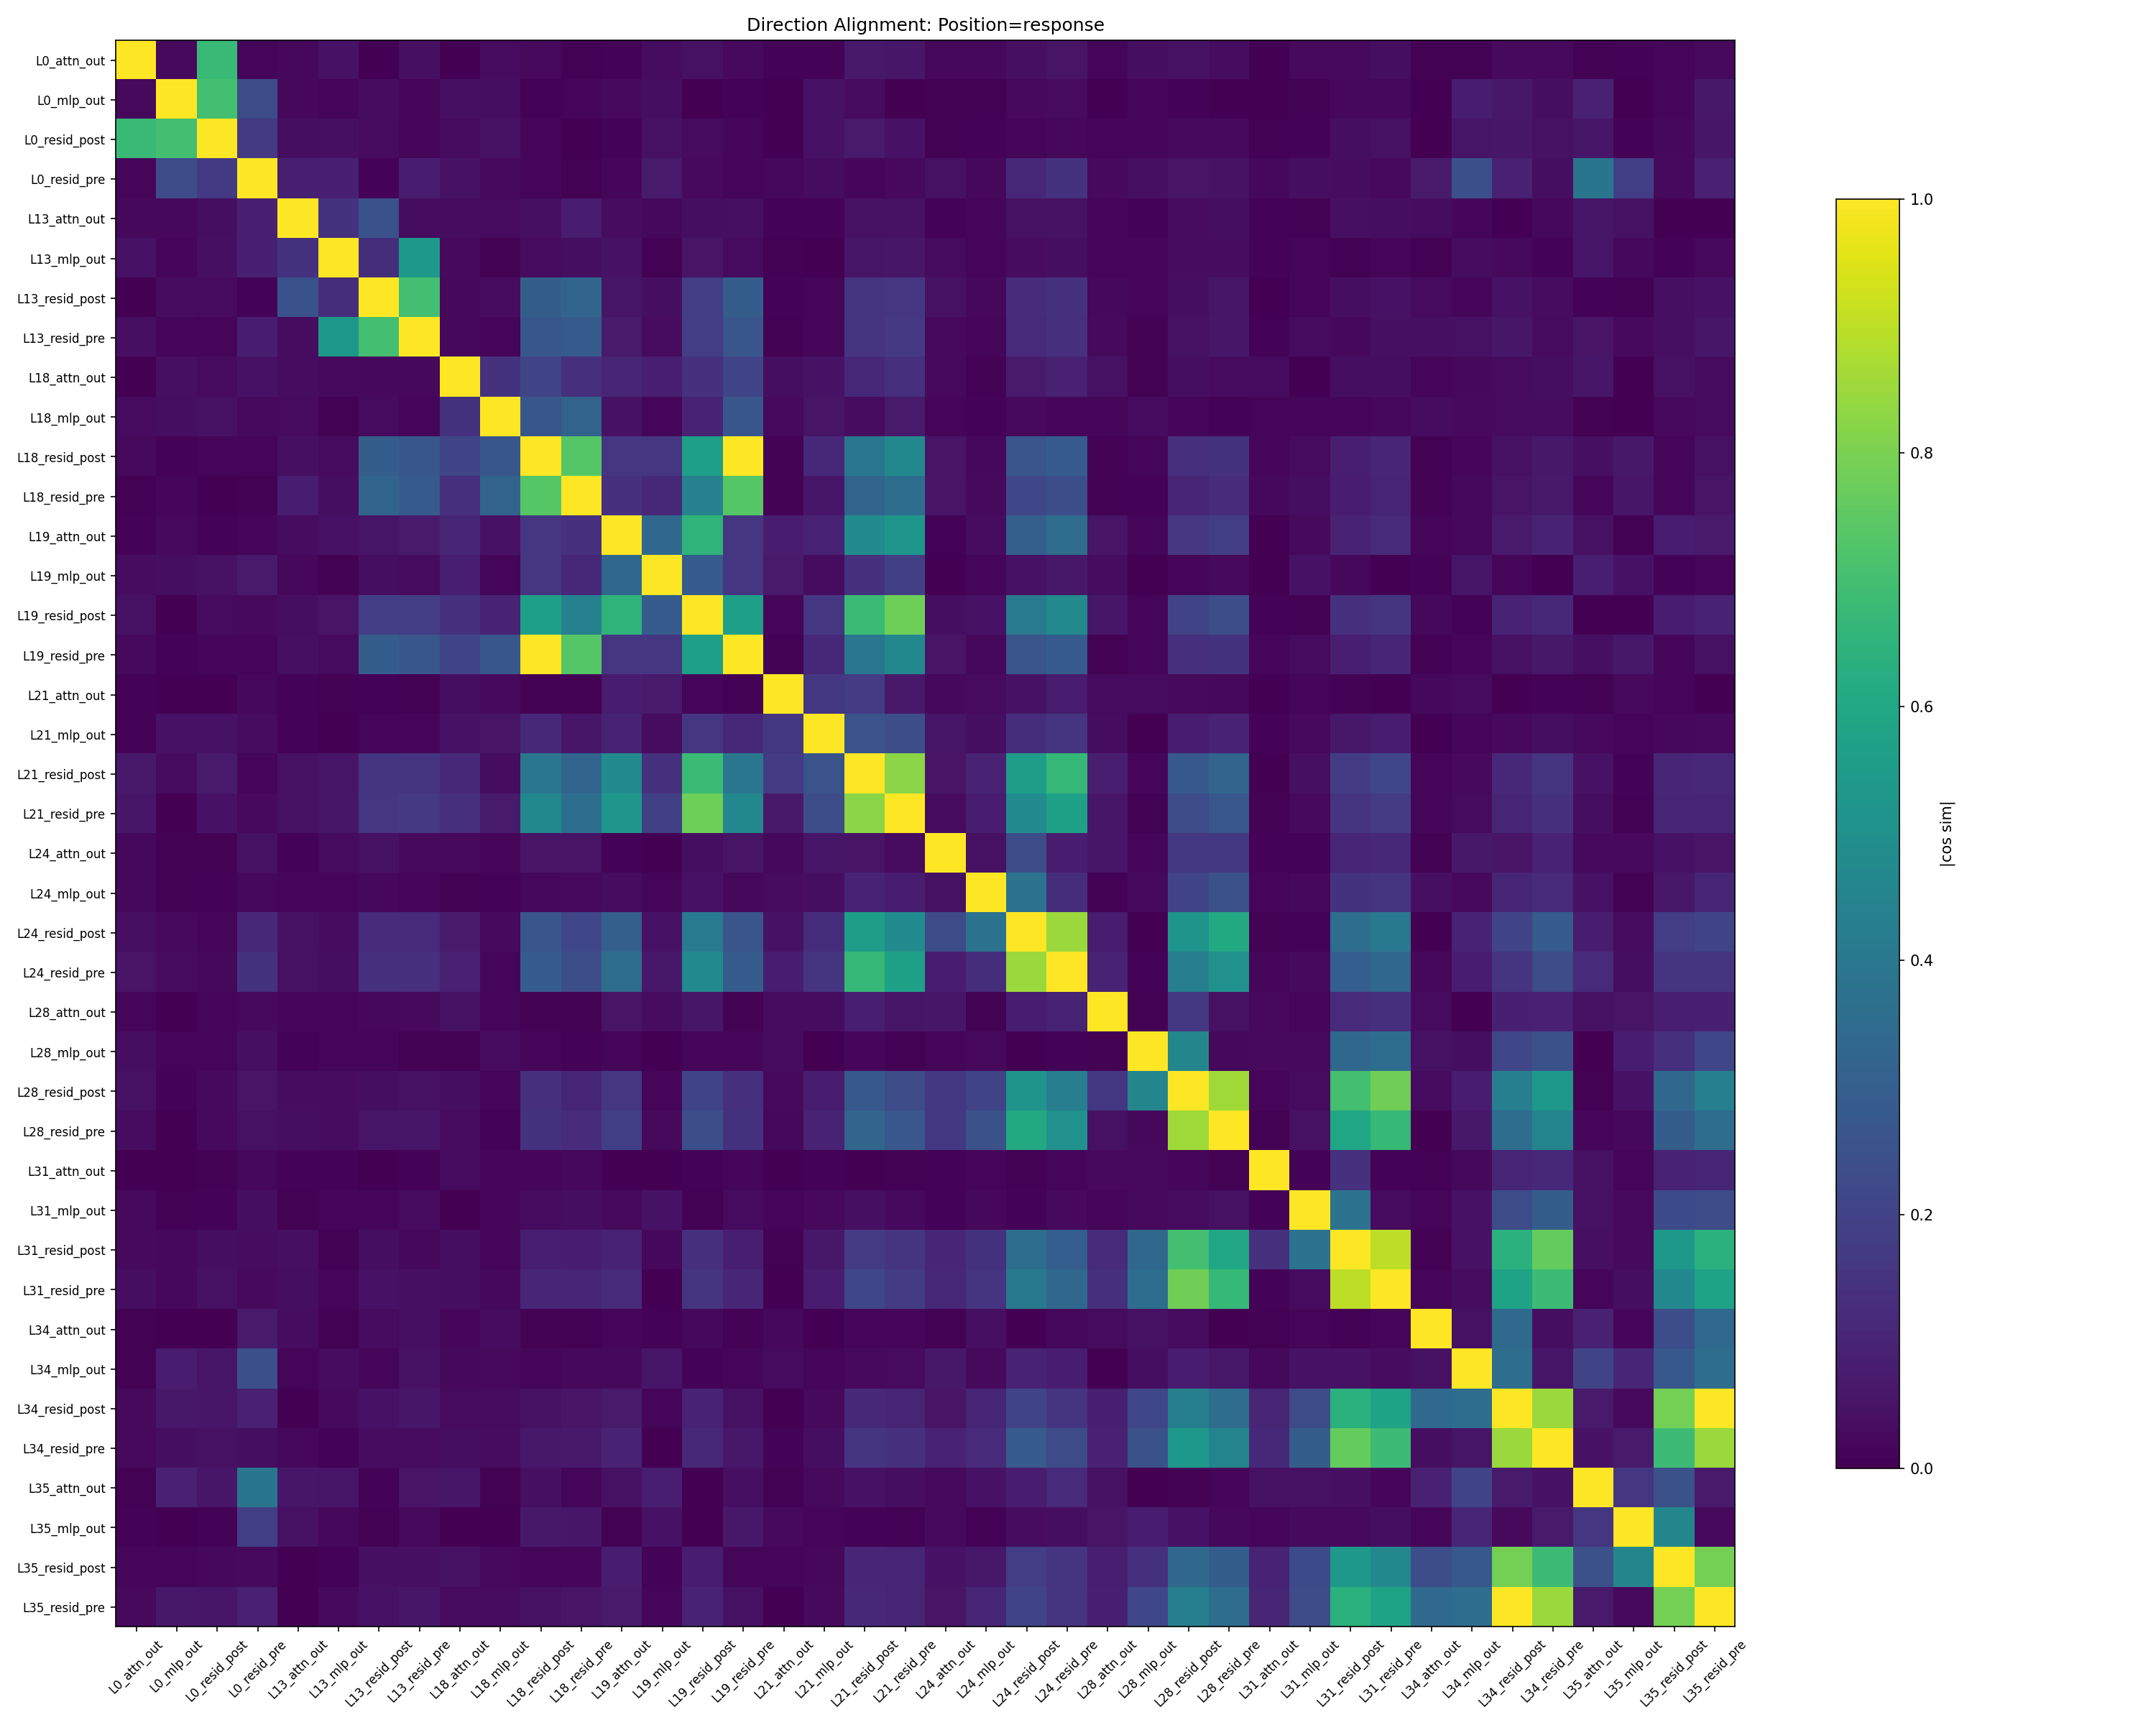
\includegraphics[width=\textwidth]{geo/direction_alignment_response.png}
\caption{Alignment to logit direction}
\end{subfigure}
\caption{Direction dynamics through the circuit. Left: Layer-to-layer cosine similarity showing stability with dips at integration points. Right: Alignment to the logit-difference direction---near-zero through processing layers until late rotation at L34--L35.}
\label{fig:direction}
\end{figure}

\begin{figure}[ht]
\centering
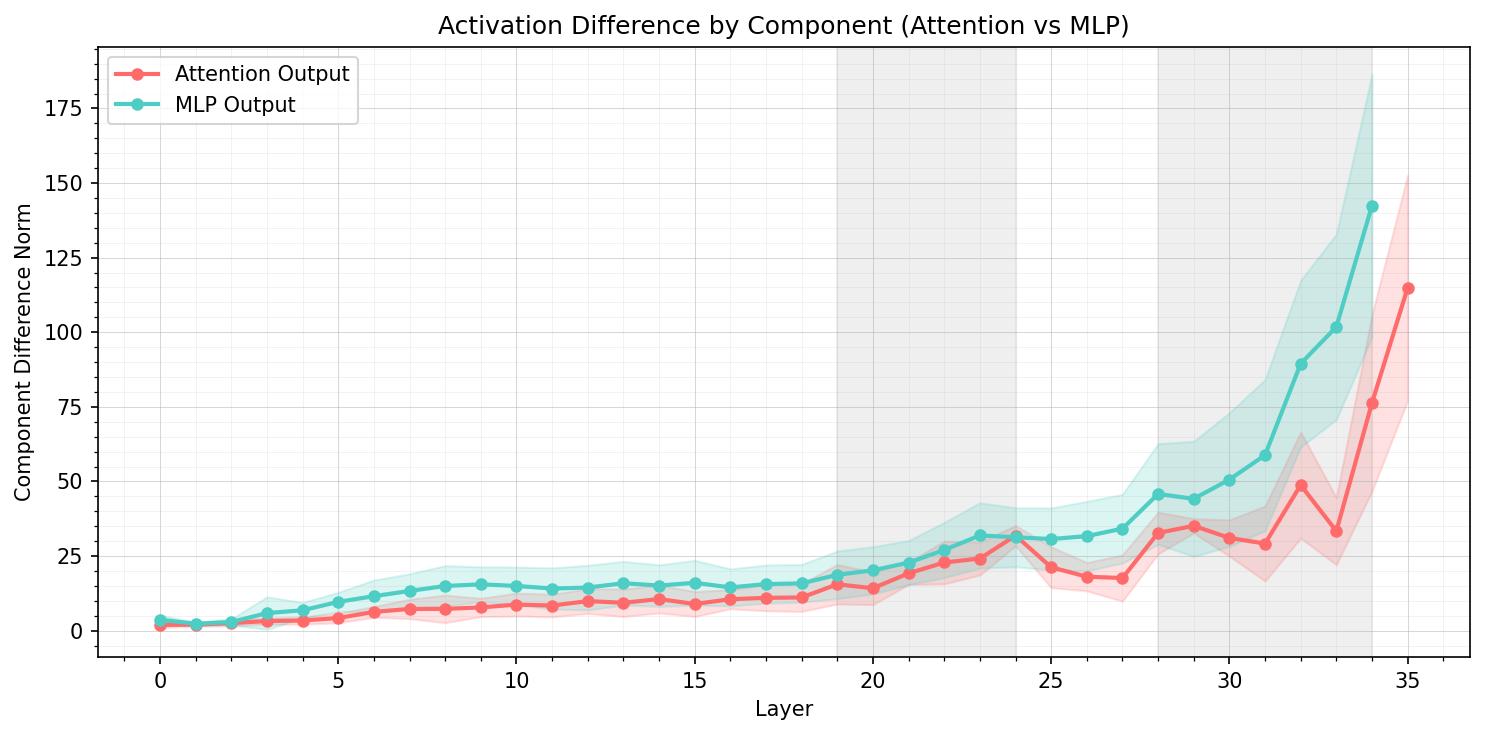
\includegraphics[width=0.7\textwidth]{diffmeans/component_norm_decomposition.png}
\caption{Component contribution to norm growth. The difference-in-means signal grows through the network with distinct contributions from attention (blue) and MLP (orange) components. MLPs dominate in late layers, consistent with their role in the Decide phase.}
\label{fig:norm_decomp}
\end{figure}

\subsection{Default Preference and Competing Circuits}
\label{sec:competing}

\subsubsection{The Default}

Without a horizon constraint, the model chooses long-term in 100\% of cases (16/16), with near-certainty. This holds regardless of reward magnitude or delivery time. The model has a \textbf{default temporal preference} that emerges when no explicit constraint is provided.

\subsubsection{Competing Circuits at L19}

L19 attention helps recovery (+0.13) but L19 MLP hurts it ($-0.10$). The EAP-IG work independently finds L19 MLP has the highest entropy. This converging evidence suggests:

\begin{itemize}
    \item \textbf{L19 MLP} encodes the default preference (favoring long-term)
    \item \textbf{L19 attention} reads the horizon constraint (which may favor short-term)
    \item When a short horizon is specified, attention must override the MLP's default
    \item When no horizon or a long horizon is given, default and constraint agree---no competition
\end{itemize}

This predicts an asymmetry: short-horizon choices require more circuit activation than long-horizon choices. The model has internalized a default temporal preference during training, likely reflecting the distribution of temporal reasoning in instructional/advisory training data that tends to favor long-term thinking.

\section{Discussion}

\paragraph{A general temporal reasoning module.} The cross-method convergence is our strongest evidence. Two completely independent approaches---structured economic choice and simple A/B temporal preference---identify the same layers, the same phasing, the same competing-circuit structure. This suggests L19--L24 is a reusable subnetwork for temporal reasoning, not a task artifact. The specificity is notable: out of 36 layers, only a contiguous band of $\sim$6 layers (17\% of the network) carries the temporal signal.

\paragraph{The Read-Refine-Decide pipeline.} The circuit is not a simple relay. Source positions carry the raw input feature; attention in L19--L24 integrates and routes it; L21 compresses redundant signals; L24 crystallizes the continuous representation; MLPs in L28--L35 threshold it into a binary decision. The asymmetric redundancy (over-reading at source, hard bottleneck at destination) is an architecturally sensible robustness strategy. Approximately 8 components account for 80\% of the effect, with L24 attention alone contributing 36\%.

\paragraph{Multi-dimensional encoding.} The model's temporal representation encodes continuous magnitude + categorical scale + binary choice in partially overlapping but distinct dimensions. This is richer than needed for the binary task and consistent with the superposition hypothesis: general features built during pre-training, repurposed for specific tasks during instruction tuning.

\paragraph{Departure from human temporal reasoning.} The model's behavior differs qualitatively from human patterns. Humans show hyperbolic discounting with magnitude effects; the model shows categorical switching with complete magnitude insensitivity. Humans exhibit preference reversals and present bias; the model shows perfect consistency within horizon conditions. The decision boundary (6 months to 2 years) may reflect training data distributions rather than any economic principle. This suggests the model learned a heuristic (``short horizons $\rightarrow$ short-term choice'') rather than a discount function.

\paragraph{Default preferences and competing circuits.} The L19 antagonism (MLP encoding default, attention reading constraint) mirrors dual-process models in behavioral economics. The model has an intrinsic long-term preference that explicit constraints must override. This is relevant to AI alignment: these hidden default preferences shape outputs when prompts are ambiguous or unconstrained, and instruction tuning appears to instill a long-term orientation (base Qwen3-4B shows 50/50 split; instruction-tuned version shows $>$85\% long-term preference).

\paragraph{Limitations.} We study a single model family (Qwen3-4B). LayerNorm-corrected logit lens has not yet been computed; the near-zero cosine to logit direction may be an artifact. Contrastive pairs partially confound horizon with reward/delivery-time variation, though our behavioral analysis shows these variables have no effect. Head-level decomposition and path patching remain future work. The competing-circuits hypothesis at L19 needs direct validation via ablation. The decision boundary location (6mo--2yr) may be specific to this model and training data.

\section{Future Work}

\paragraph{Circuit refinement.} The 2D attention geometry at L24 demands head-level decomposition---which heads encode magnitude vs.\ category? Neuron analysis at L31 ($R^2 = 0.993$) and L35 (80° rotation) MLPs could reveal interpretable features. Path patching from L24 attention to L31/L35 MLP would map causal edges.

\paragraph{Competing circuits validation.} L19 MLP ablation could test whether removing the default improves short-horizon accuracy. Geometric projection of no-horizon prompts into the PCA space could visualize where the ``default'' lives relative to explicit horizons.

\paragraph{Generalization.} Cross-model validation (Qwen3-8B, Llama, GPT-family) would test whether the L19--L24 pattern is architecture-specific or universal. Steering experiments using the identified circuit directions could enable temporal preference manipulation.

\paragraph{Interpretability.} Sparse autoencoder (SAE) analysis at L24 and L31 could decompose the multi-dimensional encoding into monosemantic features, potentially revealing human-interpretable temporal concepts.

\begin{ack}
Acknowledgments omitted for anonymous submission.
\end{ack}

\bibliographystyle{plainnat}
\bibliography{references}

%%%%%%%%%%%%%%%%%%%%%%%%%%%%%%%%%%%%%%%%%%%%%%%%%%%%%%%%%%%%

\appendix

\section{Extended Circuit Analysis}

\subsection{Redundancy Architecture}

The circuit exhibits a characteristic redundancy pattern:
\begin{itemize}
    \item \textbf{Source:} Redundant (multiple parallel readers)
    \item \textbf{Processing:} Moderately redundant (several attention layers carry overlapping information)
    \item \textbf{Destination:} Non-redundant (single output point)
\end{itemize}

This fan-out at source $\rightarrow$ converge at destination pattern is architecturally sensible. Cumulative recovery exceeds 2.0$\times$ the clean-corrupted gap, confirming substantial overlap between components.

\begin{figure}[ht]
\centering
\begin{subfigure}[b]{0.48\textwidth}

\includegraphics[width=\textwidth]{act/sweep_resid_post/position_sweep/denoising/combined.png}
\caption{Position sweep (denoising)}
\end{subfigure}
\hfill
\begin{subfigure}[b]{0.48\textwidth}

\includegraphics[width=\textwidth]{act/sweep_resid_post/position_sweep/noising/combined.png}
\caption{Position sweep (noising)}
\end{subfigure}
\caption{Position-wise patching results for \texttt{resid\_post}. Both methods identify the source hub (P73--P88) and destination bottleneck (P128--P145). Noising shows sharper destination localization; denoising shows broader source recovery---consistent with the redundancy architecture.}
\label{fig:position_sweeps}
\end{figure}

\subsection{Methodological Note: Noising vs Denoising}

Our systematic comparison reveals:
\begin{itemize}
    \item Attention layers: consistently inflated by denoising (sufficient but not necessary)
    \item MLP layers: better agreement (L31 gap $< 0.05$)
    \item \texttt{resid\_post}: closest to diagonal (most trustworthy aggregate signal)
\end{itemize}

We recommend always running both methods: trust noising for bottleneck identification, denoising for sufficiency mapping.

\begin{figure}[ht]
\centering
\begin{subfigure}[b]{0.48\textwidth}
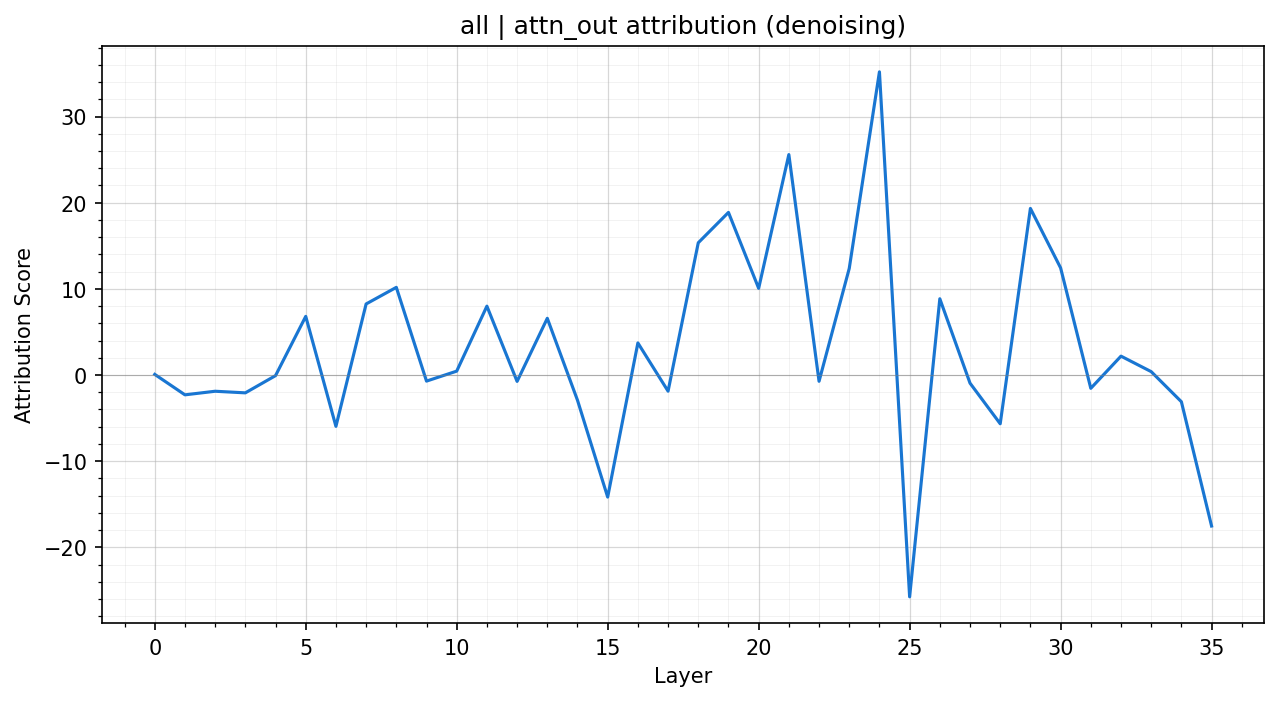
\includegraphics[width=\textwidth]{att/layer_attribution_denoising_attn_out.png}
\caption{Attention: denoising attribution}
\end{subfigure}
\hfill
\begin{subfigure}[b]{0.48\textwidth}
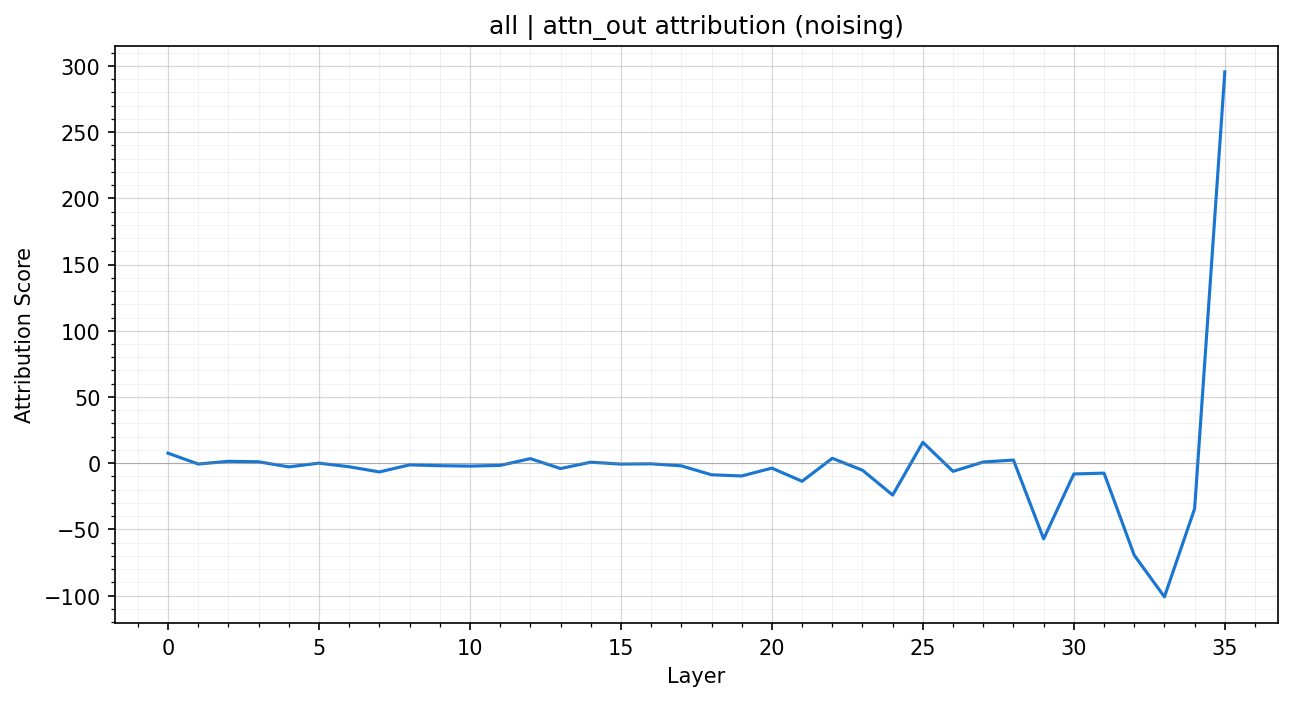
\includegraphics[width=\textwidth]{att/layer_attribution_noising_attn_out.png}
\caption{Attention: noising attribution}
\end{subfigure}
\caption{Comparison of denoising (left) and noising (right) attribution for attention layers. Denoising consistently overestimates attention importance, particularly in mid layers. The gap between methods provides information about redundancy structure.}
\label{fig:noising_denoising}
\end{figure}

\section{Behavioral Economics Connections}

\subsection{Discount Function}

Standard economic models assume agents discount future rewards:
\begin{itemize}
    \item \textbf{Exponential discounting:} $\delta^t$ (rational benchmark---constant discount rate)
    \item \textbf{Hyperbolic discounting:} $\frac{1}{1+kt}$ (behavioral economics standard---present bias)
    \item \textbf{Quasi-hyperbolic ($\beta$-$\delta$):} $\beta\delta^t$ for $t>0$ (discrete present bias)
\end{itemize}

The model's behavior fits \textbf{none of these}. Instead, we observe step-function behavior: $P(\text{long-term}) = 0$ for horizons $\leq$ 6 months, $P(\text{long-term}) = 1$ for horizons $\geq$ 2 years, with a transition zone at 7 years (56\% short-term). This categorical switching is more consistent with a learned heuristic than a discount function.

\subsection{Departures from Economic Rationality}

The model shows several qualitative departures from human economic behavior:

\begin{itemize}
    \item \textbf{Complete reward-insensitivity:} Varying reward ratios from 12$\times$ to 100$\times$ produces identical choice distributions. Humans show clear magnitude effects---larger rewards are more motivating regardless of timing.

    \item \textbf{Complete delivery-time insensitivity:} Varying delivery from 6 months to 30 years produces identical choice distributions. Humans show delay aversion---identical rewards are preferred sooner.

    \item \textbf{Framing dominance:} The horizon constraint completely determines choice. This is closer to ``frame-based reasoning'' than utility maximization.

    \item \textbf{Default long-term preference:} When unconstrained, the model always chooses the patient option (48/48 cases). This likely reflects instruction tuning on advisory text that favors long-term thinking.

    \item \textbf{Perfect consistency:} No stochasticity, no preference reversals, no context effects beyond horizon. Human choices show substantial noise and framing sensitivity.
\end{itemize}

These patterns suggest the model learned a simple decision rule (``match choice to horizon category'') rather than internalizing any economic principle. The circuit we identify implements this categorical mapping, not a discount function.

\section{Prompt Templates}

\subsection{Intertemporal Choice Format}

\begin{verbatim}
You are making a financial decision. [Context about scenario]

You are primarily concerned about outcomes in [HORIZON].

Choose one:
a) [Small-soon option]
b) [Large-later option]

Respond exactly: "I choose : a )" or "I choose : b )"
\end{verbatim}

\subsection{CAA Contrastive Pairs}

Example pairs (no economic framing):
\begin{verbatim}
Pair 1:
A: "Focus on: immediate fix"
B: "Focus on: lasting value"

Pair 2:
A: "Priority: quick results"
B: "Priority: sustainable growth"
\end{verbatim}

\section{Open-Form Temporal Preference via EAP-IG}

Independent of the structured intertemporal choice framework, we applied Edge Attribution Patching with Integrated Gradients (EAP-IG) to open-form temporal preference prompts. This methodology tests whether the same circuit mediates temporal reasoning in a completely different task format.

\subsection{Prompt Format}

The open-form prompts present a simple A/B choice without economic framing, reward magnitudes, or delivery times:

\begin{verbatim}
<|im_start|>system
You are a strategic planning assistant that follows
user instructions carefully<|im_end|>
<|im_start|>user
When deciding on a solution to this problem, you should
focus on:
 (A) What works right now to fix the immediate issue
 (B) What will create lasting value over the next decade
<|im_end|>
<|im_start|>assistant
Answer: (
\end{verbatim}

Contrastive pairs are formed by swapping the labels (A $\leftrightarrow$ B). The metric is $\text{logit}[A] - \text{logit}[B]$, where A represents short-term and B represents long-term preference.

\subsection{EAP-IG Methodology}

Standard Expected Attention Perturbation (EAP) computes attribution scores as $\text{score} = (\text{activation}) \cdot (\text{gradient at clean})$. However, components whose gradient at the clean state is near zero receive low scores even if they are causally important.

EAP-IG addresses this by computing a path integral of gradients from clean to corrupted:
\begin{equation}
\text{IntegratedGrads}_i(x) = (x_i - x'_i) \times \int_{\alpha=0}^{1} \frac{\partial F(x' + \alpha(x - x'))}{\partial x_i} d\alpha
\end{equation}

This satisfies the \textbf{completeness} property: $\sum_i \text{IntegratedGrads}_i(x) = F(x) - F(x')$, ensuring attributions sum to the actual output difference.

Following \citet{syed2023attribution}, we interpolate token embeddings (not internal activations) and use the resulting component outputs for attribution, reducing computational cost from $O(\text{n\_steps} \times \text{n\_edges})$ to $O(\text{n\_steps})$ forward passes.

\textbf{Quadrature methods.} We compared Riemann (midpoint) sum, Gauss-Legendre, and Gauss-Chebyshev quadrature. Gauss-Chebyshev produces higher average scores, identifying nodes lost to noise in other methods.

\subsection{Results: Competing Circuits}

EAP-IG reveals a striking pattern of \textbf{competing circuits}:

\begin{itemize}
    \item \textbf{Top negative scores} (opposing the logit-diff direction): Early attention layers L0, L15, L17, L21
    \item \textbf{Top positive scores} (aligned with logit-diff direction): Late MLP layers L25, L26, L27
\end{itemize}

This mirrors the competing-circuit structure found in the intertemporal choice experiments (Section~\ref{sec:competing}): attention reads contextual signals while MLPs encode default preferences.

\subsection{Cross-Model Consistency}

We applied EAP-IG across the Qwen model family (Qwen3-0.6B, Qwen2.5-1.5B, Qwen3-1.7B, Qwen3-4B, Qwen3-8B), spanning 0.6B to 8B parameters. All models show:
\begin{itemize}
    \item Non-monotonic residual stream attribution (scores decrease then increase through layers)
    \item Negative attribution at middle layers, consistent with competing circuits
    \item Similar layer-wise structure despite varying model sizes (13$\times$ parameter range)
\end{itemize}

This cross-scale consistency suggests the temporal reasoning circuit is a robust architectural pattern rather than an artifact of specific model size or training run. The relative layer positions (middle attention vs.\ late MLP) are preserved even as absolute layer counts vary.

\subsection{Selectivity}

Out of $\sim$400,000 nodes in Qwen3-4B, only $\sim$200 nodes (0.05\%) have attribution scores exceeding threshold. The identified nodes trace a connected path from input to output, indicating a coherent circuit rather than scattered noise.

\subsection{Behavioral Robustness}

\textbf{Option order consistency.} When swapping A and B positions, 83.4\% of prompts produce consistent temporal preferences, indicating the model responds to semantic content rather than position bias.

\textbf{Default preference.} Qwen3-4B-Instruct shows strong long-term preference ($>$85\% of prompts), while base Qwen3-4B shows near-equal split. This suggests instruction tuning instills a default long-term orientation.

\subsection{Convergence with Intertemporal Method}

Both methods---structured intertemporal choice (activation patching) and open-form CAA (EAP-IG)---converge on the same findings:

\begin{enumerate}
    \item \textbf{Same critical layers}: L19--L24 attention, L25--L35 MLP
    \item \textbf{Same competing-circuit structure}: Early attention with negative/opposing contribution, late MLP with positive contribution
    \item \textbf{Same default preference}: Long-term choice when unconstrained
\end{enumerate}

This convergence across completely different task formats (economic choice vs.\ simple A/B preference), corruption methods (activation patching vs.\ embedding interpolation), and metrics (recovery rate vs.\ integrated gradients) provides strong evidence for a \textbf{general temporal reasoning module} rather than task-specific artifacts.

%%%%%%%%%%%%%%%%%%%%%%%%%%%%%%%%%%%%%%%%%%%%%%%%%%%%%%%%%%%%

\section{Detailed Intertemporal Methodology}

This appendix provides comprehensive implementation details for the intertemporal preference experiment, including dataset generation, contrastive pair construction, activation patching procedures, and geometric analysis methods. We collected 122 behavioral samples across 4 datasets: a 48-sample dataset (horizons: 1yr, 10yr, none), a 64-sample dataset (horizons: 1yr, 7yr, 15yr, none), an 8-sample horizon sweep (1mo through 50yr), and a 2-sample mini dataset for rapid testing.

\subsection{Dataset Generation}

\subsubsection{Prompt Template Structure}

Prompts follow a templated question-response format with systematic variation across multiple dimensions. The base template contains:

\begin{itemize}
    \item \textbf{Context variables:} Scenario description (default: housing development), role specification (default: city administration), and reward units (default: housing units)
    \item \textbf{Option variables:} Left/right term labels, reward magnitudes, and delivery times
    \item \textbf{Horizon variable:} Time constraint (e.g., ``You are primarily concerned about outcomes in [HORIZON]'')
\end{itemize}

\subsubsection{Option Grid Generation}

For each option (short-term and long-term), we specify:
\begin{itemize}
    \item \texttt{reward\_range}: $[\text{min}, \text{max}]$ reward values (e.g., $[1000, 2500]$ for short-term, $[30000, 100000]$ for long-term)
    \item \texttt{time\_range}: $[\text{min}, \text{max}]$ delivery times with unit specification
    \item \texttt{reward\_steps}, \texttt{time\_steps}: Number of intervals and stepping type (linear or logarithmic)
\end{itemize}

\textbf{Stepping algorithms:}
\begin{itemize}
    \item Linear: $v_i = v_{\min} + i \cdot \frac{v_{\max} - v_{\min}}{n}$
    \item Logarithmic: $v_i = \exp\left(\log v_{\min} + i \cdot \frac{\log v_{\max} - \log v_{\min}}{n}\right)$
\end{itemize}

\subsubsection{Formatting Variations}

To test robustness, we optionally vary:
\begin{itemize}
    \item \textbf{Labels:} ``[A]''/``[B]'' vs ``Option 1''/``Option 2'' vs numeric alternatives
    \item \textbf{Time units:} Years, months, weeks, days
    \item \textbf{Number format:} Digits (``1000'') vs spelled out (``one thousand'')
    \item \textbf{Order:} Short-term on left vs right
\end{itemize}

Grid mode generates all combinations; random mode samples per-prompt variations.

\subsection{Contrastive Pair Construction}

\subsubsection{Preference Sample Generation}

For each prompt, we query the model and record:
\begin{itemize}
    \item \textbf{Choice:} Selected option (short-term or long-term)
    \item \textbf{Divergent logprobs:} $[\log P(a), \log P(b)]$ at the decision token
    \item \textbf{Time horizon:} Specified constraint or None
    \item \textbf{Cached activations:} Hook outputs for patching (optional)
\end{itemize}

\subsubsection{Pair Formation}

Two samples form a \textbf{contrastive pair} if:
\begin{enumerate}
    \item Sample 1 chose short-term (clean trajectory)
    \item Sample 2 chose long-term (corrupted trajectory)
    \item They differ systematically in time horizon
\end{enumerate}

The ``clean'' trajectory represents the behavior we aim to recover (short-term choice); the ``corrupted'' trajectory represents the counterfactual (long-term choice).

\subsubsection{Position Alignment}

Token positions differ between prompts due to variable-length horizon specifications (e.g., ``1 month'' vs ``50 years''). We handle this via \textbf{anchor-based position mapping}:

\begin{enumerate}
    \item Identify anchor tokens (label strings, structural markers)
    \item Build explicit mapping between clean and corrupted positions at anchors
    \item For unmapped positions, use linear interpolation: $p_{\text{dst}} = \frac{p_{\text{src}}}{L_{\text{src}}} \cdot L_{\text{dst}}$
\end{enumerate}

This ensures patching operates on semantically corresponding positions despite length differences.

\subsection{Activation Patching Implementation}

\subsubsection{Patching Modes}

We implement two complementary patching modes:

\textbf{Denoising (sufficiency test):}
\begin{itemize}
    \item Run forward pass on \textbf{corrupted} prompt (baseline)
    \item Inject \textbf{clean} activations at target layers/positions
    \item Measure: Does injecting clean circuits recover clean behavior?
\end{itemize}

\textbf{Noising (necessity test):}
\begin{itemize}
    \item Run forward pass on \textbf{clean} prompt (baseline)
    \item Inject \textbf{corrupted} activations at target layers/positions
    \item Measure: Does injecting corrupted circuits disrupt clean behavior?
\end{itemize}

\subsubsection{Component Targets}

We patch four component types via TransformerLens hooks:
\begin{itemize}
    \item \texttt{resid\_post}: Residual stream after full layer block
    \item \texttt{attn\_out}: Attention head outputs (pre-residual addition)
    \item \texttt{mlp\_out}: MLP outputs (pre-residual addition)
    \item \texttt{resid\_pre}: Residual stream before layer block
\end{itemize}

Hook names follow the pattern \texttt{blocks.\{layer\}.hook\_\{component\}}.

\subsubsection{Intervention Mechanism}

The patching intervention uses forward hooks:
\begin{enumerate}
    \item Cache source activations from clean (denoising) or corrupted (noising) forward pass
    \item Register hook on target component that replaces activations: $a_{\text{target}} \leftarrow a_{\text{source}}$
    \item Run destination forward pass with hook active
    \item Extract logits at decision position
\end{enumerate}

For position-specific patching, only the specified positions are modified; other positions pass through unchanged.

\subsubsection{Sweep Types}

\textbf{Sanity check:} Patch all layers at all positions before divergence. If full patching doesn't flip the decision, the pair is invalid.

\textbf{Layer sweep:} Fix position at divergent$-1$, vary layer ranges:
\begin{verbatim}
for layer_range in chunks(0..n_layers, step_size):
    result = patch(positions=[div_pos-1], layers=layer_range)
\end{verbatim}

\textbf{Position sweep:} Fix layers to all, vary position ranges:
\begin{verbatim}
for pos_range in chunks(start_pos..div_pos, step_size):
    result = patch(positions=pos_range, layers=ALL)
\end{verbatim}

\textbf{Key design decision:} Layer sweeps patch at position $\text{divergent}-1$ rather than all positions because the residual stream propagates information uniformly---patching all positions would obscure per-layer attribution.

\subsection{Metrics}

\subsubsection{Recovery and Disruption}

Let $y$ denote the logit difference $\log P(a) - \log P(b)$, where $a$ is the short-term option. We compute:

\textbf{Recovery} (denoising mode):
\begin{equation}
R = \frac{y_{\text{intervened}} - y_{\text{corrupted}}}{y_{\text{clean}} - y_{\text{corrupted}}}
\end{equation}

$R \in [0, 1]$: fraction of the clean-corrupted gap recovered by intervention. $R = 1$ indicates full recovery to clean behavior.

\textbf{Disruption} (noising mode):
\begin{equation}
D = \frac{y_{\text{clean}} - y_{\text{intervened}}}{y_{\text{clean}} - y_{\text{corrupted}}}
\end{equation}

$D \in [0, 1]$: fraction of clean behavior disrupted. $D = 1$ indicates complete disruption. Note: $D = 1 - R$ when both are computed from the same intervention.

\subsubsection{Redundancy Gap}

The \textbf{redundancy gap} $= R - D$ (or equivalently, denoising effect $-$ noising effect) distinguishes:
\begin{itemize}
    \item \textbf{Large positive gap:} Component is sufficient but not necessary (redundant pathway)
    \item \textbf{Near-zero gap:} Component is both necessary and sufficient (bottleneck)
    \item \textbf{Large negative gap:} Component is necessary but not sufficient (distributed processing)
\end{itemize}

\subsubsection{Fork Metrics}

At the decision position, we measure uncertainty via:

\textbf{Fork entropy} (Rényi entropy):
\begin{equation}
H_q = \frac{1}{1-q} \log \sum_i p_i^q
\end{equation}

\textbf{Fork diversity} (effective number of options):
\begin{equation}
D_q = \left(\sum_i p_i^q\right)^{1/(1-q)}
\end{equation}

For binary choices, $D_q \in [1, 2]$ where 1 indicates certainty and 2 indicates maximum uncertainty.

\subsubsection{Multilabel Aggregation}

For pairs with different label formats (multilabel mode), we aggregate across label pairs using:
\begin{itemize}
    \item \texttt{MEAN\_NORMALIZED}: Arithmetic mean after softmax (default)
    \item \texttt{MEAN\_LOGPROB}: Arithmetic mean of log probabilities
    \item \texttt{SUM\_LOGPROB}: Log-sum-exp aggregation
\end{itemize}

\subsection{Geometric Analysis}

\subsubsection{Activation Collection}

We extract activations at specified hook points (\texttt{resid\_pre}, \texttt{resid\_post}, \texttt{mlp\_out}, \texttt{attn\_out}) for all layers and semantic positions:
\begin{itemize}
    \item \textbf{Source positions:} \texttt{time\_horizon}, \texttt{short\_term\_time}, \texttt{short\_term\_reward}, \texttt{long\_term\_time}, \texttt{long\_term\_reward}
    \item \textbf{Destination positions:} \texttt{response} (decision token)
\end{itemize}

Position resolution uses substring matching in tokenized text to locate value mentions.

\subsubsection{PCA Methodology}

For each (layer, component, position) tuple:
\begin{enumerate}
    \item Fit PCA on activation matrix $X \in \mathbb{R}^{n \times d}$ where $n$ = samples, $d$ = model dimension
    \item Extract explained variance ratios for each PC
    \item Compute Spearman correlation between each PC and $\log_{10}(\text{time horizon})$
    \item Store top 20 components for analysis
\end{enumerate}

\textbf{Configuration:} 50 components fitted, no explicit scaling, random seed 42.

\subsubsection{Linear Probe Implementation}

We train Ridge regression probes ($\alpha = 10.0$) to predict $\log_{10}(\text{time horizon months} + 1)$ from activations:

\begin{enumerate}
    \item Pipeline: StandardScaler $\rightarrow$ Ridge($\alpha=10.0$)
    \item Cross-validation: $k = \min(5, n/2)$ folds, stratified shuffle
    \item Metric: $R^2$ (can be negative if worse than mean prediction)
\end{enumerate}

\textbf{Interpretation:} High $R^2$ indicates the layer explicitly encodes temporal magnitude; low $R^2$ suggests implicit or distributed encoding.

\subsubsection{Direction Stability Analysis}

For each layer, we compute the difference-in-means vector:
\begin{equation}
\Delta_L = \frac{1}{n}\sum_i (a_i^{\text{clean}} - a_i^{\text{corrupted}})_L
\end{equation}

\textbf{Metrics:}
\begin{itemize}
    \item \textbf{Layer-to-layer cosine:} $\cos(\Delta_L, \Delta_{L+1})$ measures direction consistency
    \item \textbf{Cosine to logit:} $\cos(\Delta_L, W_U[:, a] - W_U[:, b])$ measures alignment to task direction
    \item \textbf{Norm:} $\|\Delta_L\|_2$ measures signal magnitude
\end{itemize}

\subsubsection{Rotation Decomposition}

For each layer's residual stream evolution ($\text{resid\_post} = \text{resid\_pre} + \text{attn\_out} + \text{mlp\_out}$), we decompose rotation angles:

\begin{itemize}
    \item \textbf{Attention rotation:} Angle between $\Delta(\text{resid\_pre})$ and $\Delta(\text{resid\_pre} + \text{attn\_out})$
    \item \textbf{MLP rotation:} Angle between $\Delta(\text{resid\_pre} + \text{attn\_out})$ and $\Delta(\text{resid\_post})$
    \item \textbf{Total rotation:} Angle between $\Delta(\text{resid\_pre})$ and $\Delta(\text{resid\_post})$
\end{itemize}

Angles computed via $\theta = \arccos(\text{clamp}(\cos(\cdot), -1, 1))$ and reported in degrees.

\subsubsection{Logit Lens}

We track how predictions evolve across layers using the logit lens:

\begin{equation}
\text{logit\_diff}_L = \text{LayerNorm}(\text{resid\_post}_L) \cdot W_U[:, a] - \text{LayerNorm}(\text{resid\_post}_L) \cdot W_U[:, b]
\end{equation}

\textbf{Critical implementation detail:} The final LayerNorm must be applied before projection to $W_U$, as the unembedding matrix expects normalized input.

\subsection{Reproducibility}

\subsubsection{Caching Strategy}

Results are cached per-pair and per-component, enabling:
\begin{itemize}
    \item Incremental computation (rerun only new pairs)
    \item Component independence (analyze different components separately)
    \item Visualization regeneration (replot without recomputation)
\end{itemize}

\subsubsection{Key Parameters}

\begin{table}[h]
\centering
\small
\begin{tabular}{lll}
\toprule
Parameter & Value & Rationale \\
\midrule
Ridge $\alpha$ & 10.0 & Strong regularization for high-dimensional data \\
PCA components & 50 (stored: 20) & Balance coverage and storage \\
CV folds & $\min(5, n/2)$ & Stability vs test set size \\
Random seed & 42 & Reproducibility \\
Data type & float32 & Memory efficiency \\
Buffer size & 100 samples & Streaming extraction \\
\bottomrule
\end{tabular}
\caption{Key implementation parameters.}
\label{tab:parameters}
\end{table}

All code is available at [URL redacted for anonymous submission].

%%%%%%%%%%%%%%%%%%%%%%%%%%%%%%%%%%%%%%%%%%%%%%%%%%%%%%%%%%%%

\section{Detailed Behavioral Analysis}
\label{sec:behavioral_appendix}

This appendix provides comprehensive behavioral data from our intertemporal choice experiments, including breakdowns by time horizon, reward magnitude, and delivery time.

\subsection{Horizon Sweep: Identifying the Decision Boundary}

To precisely locate the model's decision boundary, we tested 8 time horizons from 1 month to 50 years.

\begin{table}[h]
\caption{Model choice behavior across fine-grained time horizons ($n=8$ prompts, horizon sweep dataset). The decision boundary lies between 6 months (100\% short-term) and 2 years (100\% long-term).}
\label{tab:horizon_sweep}
\centering
\begin{tabular}{lccccc}
\toprule
Horizon & $n$ & Short-term & Long-term & Rational & Choice Prob \\
\midrule
1 month & 1 & 100\% & 0\% & 100\% & $>$99.99\% \\
6 months & 1 & 100\% & 0\% & 100\% & $>$99.99\% \\
\midrule
2 years & 1 & 0\% & 100\% & 100\% & $>$99.99\% \\
5 years & 1 & 0\% & 100\% & 100\% & $>$99.99\% \\
10 years & 1 & 0\% & 100\% & 100\% & $>$99.99\% \\
30 years & 1 & 0\% & 100\% & 100\% & $>$99.99\% \\
50 years & 1 & 0\% & 100\% & 100\% & $>$99.99\% \\
\midrule
No horizon & 1 & 0\% & 100\% & N/A & 86.7\% \\
\bottomrule
\end{tabular}
\end{table}

The sharp boundary between 6 months and 2 years suggests the model has learned a categorical distinction between ``short-term'' (sub-year) and ``long-term'' (multi-year) horizons, rather than a continuous discount function.

\subsection{Extended Horizon Analysis}

\begin{table}[h]
\caption{Choice behavior by time horizon across two datasets: 48-sample dataset (horizons: 1yr, 10yr, none) and 64-sample dataset (horizons: 1yr, 7yr, 15yr, none).}
\label{tab:extended_horizon}
\centering
\begin{tabular}{lcccccc}
\toprule
Horizon & Dataset & $n$ & Short-term & Long-term & Rational & Associated \\
\midrule
1 year & 48-sample & 16 & 100\% & 0\% & 100\% & 100\% \\
1 year & 64-sample & 16 & 100\% & 0\% & 100\% & 100\% \\
\midrule
7 years & 64-sample & 16 & 56.2\% & 43.8\% & 56.2\% & 93.8\% \\
\midrule
10 years & 48-sample & 16 & 0\% & 100\% & 0\% & 50\% \\
15 years & 64-sample & 16 & 0\% & 100\% & 50\% & 50\% \\
\midrule
No horizon & 48-sample & 16 & 0\% & 100\% & N/A & 0\% \\
No horizon & 64-sample & 16 & 0\% & 100\% & N/A & 0\% \\
\bottomrule
\end{tabular}
\end{table}

The 7-year horizon is the only condition showing non-unanimous choice (56.2\% short-term), confirming it lies in the transition zone between short and long-term categorization. The ``Associated'' column indicates whether the choice matches the delivery time closest to the horizon---note that even when choices are unanimous, association varies based on specific delivery times in each prompt.

\subsection{Reward Insensitivity}

\begin{table}[h]
\caption{Choice behavior by reward magnitude (64-sample dataset). Neither short-term nor long-term reward magnitude affects choice distribution.}
\label{tab:reward_sensitivity}
\centering
\begin{tabular}{lcccc}
\toprule
\multicolumn{5}{c}{\textbf{By Short-Term Reward}} \\
\midrule
Reward & $n$ & Short-term & Long-term & Rational \\
\midrule
\$1,000 & 32 & 40.6\% & 59.4\% & 53.1\% \\
\$2,500 & 32 & 37.5\% & 62.5\% & 50.0\% \\
\midrule
\multicolumn{5}{c}{\textbf{By Long-Term Reward}} \\
\midrule
Reward & $n$ & Short-term & Long-term & Rational \\
\midrule
\$30,000 & 32 & 37.5\% & 62.5\% & 50.0\% \\
\$100,000 & 32 & 40.6\% & 59.4\% & 53.1\% \\
\midrule
\multicolumn{5}{c}{\textbf{By Reward Ratio (long/short)}} \\
\midrule
Ratio & $n$ & Short-term & Long-term & Rational \\
\midrule
12$\times$ & 16 & 37.5\% & 62.5\% & 50.0\% \\
30$\times$ & 16 & 37.5\% & 62.5\% & 50.0\% \\
40$\times$ & 16 & 37.5\% & 62.5\% & 50.0\% \\
100$\times$ & 16 & 43.8\% & 56.2\% & 56.2\% \\
\bottomrule
\end{tabular}
\end{table}

The variation in choice percentages across reward levels is entirely explained by the horizon distribution within each reward condition---controlling for horizon, reward magnitude has zero effect. An 8$\times$ change in reward ratio (12$\times$ to 100$\times$) produces only a 6.3 percentage point change in short-term choice, all attributable to horizon composition.

\subsection{Delivery Time Insensitivity}

\begin{table}[h]
\caption{Choice behavior by delivery time (64-sample dataset). Neither short-term nor long-term delivery time affects choice distribution.}
\label{tab:time_sensitivity}
\centering
\begin{tabular}{lcccc}
\toprule
\multicolumn{5}{c}{\textbf{By Short-Term Delivery Time}} \\
\midrule
Delivery & $n$ & Short-term & Long-term & Rational \\
\midrule
6 months & 32 & 37.5\% & 62.5\% & 50.0\% \\
1 year & 32 & 40.6\% & 59.4\% & 53.1\% \\
\midrule
\multicolumn{5}{c}{\textbf{By Long-Term Delivery Time}} \\
\midrule
Delivery & $n$ & Short-term & Long-term & Rational \\
\midrule
10 years & 32 & 37.5\% & 62.5\% & 50.0\% \\
30 years & 32 & 40.6\% & 59.4\% & 53.1\% \\
\bottomrule
\end{tabular}
\end{table}

Tripling the long-term delivery time (10 to 30 years) has no effect on choice behavior---the model responds to the horizon constraint, not the actual temporal structure of the options.

\subsection{Cross-Dataset Consistency}

\begin{table}[h]
\caption{Summary statistics across all datasets. The model shows consistent behavioral patterns across different prompt configurations.}
\label{tab:cross_dataset}
\centering
\begin{tabular}{lccccc}
\toprule
Dataset & $n$ & Short-term & Long-term & Rational & Confidence \\
\midrule
48-sample & 48 & 33.3\% & 66.7\% & 33.3\% & $>$99.99\% \\
64-sample & 64 & 39.1\% & 60.9\% & 51.6\% & $>$99.99\% \\
Horizon sweep & 8 & 25.0\% & 75.0\% & 87.5\% & $>$86.7\% \\
Mini (2) & 2 & 50.0\% & 50.0\% & 100.0\% & $>$99.99\% \\
\midrule
\textbf{Combined} & 122 & 35.2\% & 64.8\% & 47.5\% & --- \\
\bottomrule
\end{tabular}
\end{table}

The variation in overall short-term percentage (25\%--50\%) is entirely explained by the horizon distribution in each dataset. Within matched horizon conditions, choice behavior is perfectly consistent across datasets.

\subsection{Confidence and Decision Certainty}

All decisions are made with extreme confidence. The typical choice probability is $>$99.99\%, corresponding to logit differences of 20+ in favor of the chosen option. The only exception is the no-horizon condition in the horizon sweep dataset, where confidence drops to 86.7\%---still decisive, but noticeably less certain than when an explicit horizon is provided. This suggests the model's ``default'' long-term preference is less crystallized than its horizon-constrained choices.

\subsection{Summary of Behavioral Findings}

\begin{enumerate}
    \item \textbf{Categorical, not continuous:} The model treats temporal horizons as categories (short/long), not as a continuous discount function.
    \item \textbf{Sharp boundary:} The decision boundary lies between 6 months and 2 years, with 7 years as a transition zone.
    \item \textbf{Horizon dominance:} The horizon constraint completely determines choice; reward magnitude and delivery time have no effect.
    \item \textbf{Default preference:} Without a horizon constraint, the model defaults to long-term choice with slightly reduced confidence.
    \item \textbf{Perfect consistency:} Matched conditions across datasets produce identical behavior.
\end{enumerate}

These behavioral patterns---categorical processing, framing dominance, reward insensitivity---depart sharply from normative economic models and human behavioral patterns, suggesting the circuit we identify in the main text implements a qualitatively different decision mechanism.

%%%%%%%%%%%%%%%%%%%%%%%%%%%%%%%%%%%%%%%%%%%%%%%%%%%%%%%%%%%%

\newpage
\input{checklist.tex}

\end{document}
